\documentclass[10pt,superscriptaddress,
amsmath,aps,prc,twocolumn,nofootinbib,floatfix]{revtex4-1}
\ifdefined\DeclareUnicodeCharacter
  \DeclareUnicodeCharacter{03C9}{$\omega$}
  \DeclareUnicodeCharacter{03C3}{$\sigma$}
\fi

\usepackage{amssymb}  % \gtrsim, \geqslant, etc: see amsguide.ps
\usepackage{graphicx}
\usepackage{exscale}
\graphicspath{{Hydrodynamical combustion/}}
\usepackage{textcomp}
\usepackage{enumerate}
\usepackage{enumitem}
%\usepackage[spanish]{babel}
\usepackage{amsmath}
\usepackage{empheq}
\usepackage{amssymb}
%\usepackage[compat=1.1.0]{tikz-feynhand} 
\usepackage{multirow}
\usepackage{orcidlink}
%\usepackage{float}
\usepackage{subcaption}
\usepackage{float}
%\usepackage{cite}
%\usepackage{bm}
% \addtolength{\topmargin}{2cm}
%\usepackage[utf8]{inputenc}
%\usepackage[T1]{fontenc}

%%%%%%%%%%%%%%%%%%%%%%%%%%%%%%%%%%%%%%%%%%%%%%%%%%%%%%%%%%%%%%%%%
%%    This is our standard definitions of abbreviations        %%
%%%%%%%%%%%%%%%%%%%%%%%%%%%%%%%%%%%%%%%%%%%%%%%%%%%%%%%%%%%%%%%%%

\usepackage{color}
\newcommand{\com}[1]{{\sf\color[rgb]{0,0,1}[#1]}}
% Marking old and new text:
\usepackage[normalem]{ulem}  % \sout{old text} for strikeout
\newcommand{\mga}[1]{{\color[rgb]{0.6,0,0}#1}}
\newcommand{\mgacom}[1]{\textsf{\color[rgb]{0.8,0,0}[\textsuperscript{MGA} #1]}}
%\newcommand{\new}[1]{#1}
\newcommand{\old}[1]{{\color[rgb]{0.7,0.7,0.7}\sout{#1}}}
\newcommand{\new}[1]{{\color[rgb]{0.0,0.5,0.2}#1}}

\newcommand{\AH}[1]{{\color{cyan}#1}}
\newcommand{\AHcom}[1]{\textsf{\color{cyan}{\textsuperscript{AH}#1}}}

\newcommand{\LB}[1]{{\color{blue}#1}}
\newcommand{\LBcom}[1]{\textsf{\color{blue}[\textsuperscript{LB}#1]}}

\newcommand{\JS}[1]{{\color{violet}#1}}
\newcommand{\JScom}[1]{\textsf{\color{violet} [\textsuperscript{JS}#1]}}

%%%%%%%%%% Journal Styles for APS
%\newcommand\NCA{Nuovo Cimento}
%\newcommand\NPBPS{{Nucl. Phys.} B (Proc. Suppl.)}
%\newcommand\RMP{Rev. Mod. Phys.}
%\newcommand\PTP{{Prog. Theor. Phys.}}
%\newcommand\PTPS{{Prog. Theor. Phys. Suppl.}}
%\newcommand\ZPA{{Z. Phys.} A}
%\newcommand\EPJA{{Eur. Phys. J.} A}
\newcommand{\AP}[3]{Ann.\ Phys.\ {\bf #1},\ #2 (#3)}
\newcommand{\NPA}[3]{Nucl.\ Phys.\ {\bf A#1},\ #2 (#3)}
\newcommand{\NPB}[3]{Nucl.\ Phys.\ {\bf B#1},\ #2 (#3)} 
\newcommand{\PLA}[3]{Phys.\ Lett.\ A\ {\bf #1},\ #2 (#3)}
\newcommand{\PLB}[3]{Phys.\ Lett.\ B\ {\bf #1},\ #2 (#3)}
\newcommand{\PR}[3]{Phys.\ Rep.\ {\bf #1},\ #2 (#3)}
\newcommand{\PRL}[3]{Phys.\ Rev.\ Lett.\ {\bf #1},\ #2 (#3)}
\newcommand{\PRB}[3]{Phys.\ Rev.\ B\ {\bf #1},\ #2 (#3)}
\newcommand{\PRC}[3]{Phys.\ Rev.\ C\ {\bf #1},\ #2 (#3)}
\newcommand{\PRD}[3]{Phys.\ Rev.\ D\ {\bf #1},\ #2 (#3)}
\newcommand{\JPG}[3]{J.\ Phys.\ G\ {\bf #1},\ #2 (#3)}
\newcommand{\RPP}[3]{Rep.\ Prog.\ Phys.\ {\bf #1},\ #2 (#3)}
\newcommand{\ZPC}[3]{Z.\ Phys.\ C\ {\bf #1},\ #2 (#3)}
\newcommand{\EPJC}[3]{Eur.\ Phys.\ J.\ C\ {\bf #1},\ #2 (#3)}
\newcommand{\PPNP}[3]
{Prog.\ Part.\ Nucl.\ Phys.\ {\textbf #1},\ #2 (#3)}
\newcommand{\APPB}[3]{Acta.\ Phys.\ Polon.\ B\ {\bf #1},\ #2 (#3)}

\newcommand{\ibid}[3]{{\bf #1},\ #2 (#3)}
%%%%%%%%%% End Journal Definitions

%%%%%%%%%% Greek alphabets
\renewcommand\a{\alpha}
\renewcommand\b{\beta}
\newcommand\g{\gamma}
\renewcommand\d{\delta}
\newcommand\e{\epsilon}
\newcommand\ve{\varepsilon}
\newcommand\z{\zeta}
\newcommand\q{\theta}
\renewcommand\i{\iota}
\renewcommand\k{\kappa}
\renewcommand\l{\lambda}
%\newcommand\m{\mu}
\newcommand\n{\nu}
\newcommand\x{\xi}
%\newcommand\p{\pi}
\newcommand\rr{\rho}
%\newcommand\s{\sigma}
\renewcommand\t{\tau}
\renewcommand\u{\upsilon}
\newcommand\f{\phi}
\renewcommand\c{\chi}
\renewcommand\j{\psi}
\renewcommand\o{\omega}

\newcommand{\al}{\alpha}
\newcommand{\be}{\beta}
\newcommand{\ga}{\gamma}
\newcommand{\Ga}{\Gamma}
\newcommand{\de}{\delta}
\newcommand{\De}{\Delta}
\newcommand{\ep}{\varepsilon}

\newcommand{\eps}{\epsilon}
\newcommand{\ze}{\zeta}
\newcommand{\ka}{\kappa}
\newcommand{\la}{\lambda}
\newcommand{\La}{\Lambda}
\newcommand{\ph}{\varphi}
\newcommand{\del}{\nabla}
\newcommand{\si}{\sigma}
\newcommand{\Si}{\Sigma}
\renewcommand{\th}{\theta}   % LaTeX: \th already defined
\newcommand{\Up}{\Upsilon}
\newcommand{\om}{\omega}
\newcommand{\Om}{\Omega}

%%%%%%%%%% End Greek alphabets

%%%  A few capitals
\newcommand\D{\Delta}
\newcommand\G{\Gamma}
\renewcommand\L{\Lambda}
\newcommand\J{\Psi}
\newcommand\U{\Upsilon}

%%%%%%%%%%  Some abbreviations

%\newcommand{\Del}{\nabla}
%\newcommand{\eqn}[1]{(\ref{#1})}
%\newcommand{\sliver}{\kern 0.07em} % like italic correction \/
\newcommand{\dsp}{\displaystyle}
\newcommand{\hide}[1]{}
\newcommand{\m}{\text{m}}
\newcommand{\km}{\text{km}}
\newcommand{\s}{\text{s}}
\newcommand{\gram}{\text{g}}
\newcommand{\MeV}{\text{MeV}}
\newcommand{\GeV}{\text{GeV}}
\newcommand{\kHz}{\text{kHz}}
\newcommand{\Hz}{\text{Hz}}
\newcommand{\nsat}{\ensuremath{n_{0}}}
\newcommand{\Bratio}{\lambda_n}
\newcommand{\tfinal}{\ensuremath{t_\text{eq}}}
\newcommand{\azp}{\ensuremath{a(0^+)}}

%\newcommand{\half} {{\textstyle \frac{1}{2}}}
%\newcommand\deriv[3]{{\dfrac{\partial #1}{\partial #2}}\biggr|_{#3}}
%\newcommand{\p}{\partial}


\begin{document}

\title{Quark Matter Phase Boundary Evolution in Neutron Star Mergers}
 \author{M.~G.~Alford \,\orcidlink{0000-0001-9675-7005}}
 \email{alford@physics.wustl.edu}
 \affiliation{Department of Physics, Washington University in St.~Louis, St.~Louis, MO 63130, USA}
 \author{L.~Brodie\,\orcidlink{0000-0001-7708-2073}}
 \email{b.liam@wustl.edu}
 \affiliation{Department of Physics, Washington University in St.~Louis, St.~Louis, MO 63130, USA}
 \author{A.~Haber\,\orcidlink{0000-0002-5511-9565}}
 \email{alexander.haber@tuwien.ac.at}
  \affiliation{Institute for Theoretical Physics, TU Wien, 1040 Vienna, Austria}
 \affiliation{Mathematical Sciences and STAG Research Centre,
University of Southampton, Southampton SO17 1BJ, United Kingdom}
 \affiliation{Department of Physics, Washington University in St.~Louis, St.~Louis, MO 63130, USA}
 \author{J. Shao\,\orcidlink{0009-0004-9698-0177}}
 \email{jan.shao@wustl.edu}
 \affiliation{Department of Physics, Washington University in St.~Louis, St.~Louis, MO 63130, USA}
 \affiliation{McDonnell Center for the Space Sciences, Washington University in St.~Louis, St.~Louis, MO 63130, USA}

\date{\today}

\begin{abstract}
Place holder
\end{abstract}

\maketitle

\section{Introduction}

At sufficiently high densities, nuclear matter is theorized to undergo a phase transition to deconfined quark matter. While the exact nature of the phase transition is unknown, one frequently invoked scenario is a first-order phase transition with a high surface tension, leading to a sharp interface between nuclear matter and quark matter. 
%In this scenario, the phase transition occurs at a (unknown) critical pressure with a discontinuity in the energy density, determining the location and strength of the phase transition. 
Such a transition might occur 
in several astrophysical scenarios, ranging from core-collapse supernovae to isolated neutron stars and binary neutron star mergers. There has been a significant effort to develop signatures of a first order phase transition in these systems, in the gravitational or electromagnetic waves emitted, so that we can extract from observations information about the phase structure of dense matter.

Various signatures have been proposed. For example, during inspiral, a phase boundary between nuclear and quark matter may support interface modes whose excitation produces signatures that are potentially within reach of next-generation detectors like Cosmic Explorer or the Einstein Telescope \cite{Counsell:2025hcv,Pereira:2025xsi}. %The existence and frequency of the interface mode critically depend on the conversion timescale, i.e.,~the speed with which the phase boundary between nuclear and quark matter can move via conversion of metastable nuclear matter to quark matter, or vice versa. If the phase boundary can move too fast, the restoring force for the interface mode and thus the mode itself vanish. All recent analyses \cite{Tonetto:2020bie,Counsell:2025hcv,Pereira:2025xsi}  set this velocity to zero and assume that on the millisecond timescale of the oscillation, the phase content is frozen.

In the post-merger phase, there are also possible signatures of
a nuclear-quark phase boundary.
Several recent works have addressed this question using model equations of state that include a nuclear/quark transition \cite{Most:2018eaw,Bauswein:2018bma,Espino:2023llj,Weih:2019xvw,Harada:2023eyg,Bauswein:2020ggy,Haque:2022dsc,Fujimoto:2022xhv,Christian:2023hez,Fujimoto:2024ymt},
looking for features of the gravitational wave emission arising from the redistribution of mass
as regions of the denser phase grow or shrink in response to pressure gradients in the violent collision between the stars. %Current simulations assume that if a region of nuclear matter is compressed to a pressure above the critical pressure $p_\text{crit}$ where quark matter becomes favored, it will immediately convert to quark matter, so there will be no significant regions of metastable nuclear matter or out-of-equilibrium quark matter \AHcom{we need to verify this as Veronica's EOS that the Most PRL uses does have out-of-equilibrium QM}. This assumes that the phase boundary can travel distances of order kilometers in milliseconds, i.e., at speeds of order $10^6\,\m\s^{-1}$. Our results will show that this assumption is questionable.

The same phase transition may also power core-collapse supernovae: if the collapsing core of a massive star reaches the density where nuclear matter converts to quark matter, the resulting quark core can trigger a delayed second shock and explode stars that neutrino heating alone fails to explode \cite{Fischer:2010wp,Fischer:2017lag,Fischer:2021tvv}.

In isolated neutron stars, spin-down-induced compression may lead to the formation of a quark-matter core or to the growth of an existing one \cite{Glendenning:1997fy, Prasad:2022dom}. Depending on the conversion dynamics, this growth may proceed gradually or through discrete episodes involving metastable hadronic matter, potentially producing observable timing irregularities such as pulsar glitch-like events \cite{Zdunik:2006uw}.

\mga{
In all of these scenarios, a key parameter is the speed at which the nuclear/quark phase boundary can move.
Specifically, when the pressure in the vicinity of
an existing phase boundary rises above the critical pressure, how fast can the quark matter region expand, converting the metastable nuclear matter to quark matter? The propagation speed of the
phase boundary} has a profound impact on the physical outcome and observational signatures. However, in all of the cited studies, it has been treated in one of two extreme limits: the speed is assumed to be either zero or infinite.

The propagation of a nuclear/quark phase boundary has been analyzed before, mostly for the more extreme case of the conversion of hadronic stars into strange stars in the context of the strange matter hypothesis \cite{Olinto:1986je,Horvath:1988nb,Heiselberg:1991px,Lugones:1994xg,Leahy:2007we,Pagliara:2013tza,Alford:2014jha,Drago:2015fpa,Furusawa:2015vfn,Niebergal:2010ds,Ouyed:2022toz} 
This paper complements earlier work by studying a pressure driven transition to quark matter (rather than the global instability assumed by the strange matter hypothesis), giving a survey of how the boundary speed varies as a function of the density and temperature of the nuclear phase under the conditions typical of neutron star mergers (inspiral and post merger) and supernovas, and providing approximate analytic expressions for the boundary speed.
To achieve this, we adopt a simplified model, focusing on the dominant flavor equilibration channel in quark matter. We do not consider the reverse process, conversion of quark matter to nuclear matter, although this may also occur in situations where there are pressure oscillations.  We aim to set an approximate upper bound on the propagation speed of the boundary, so our approximations and simplifications are chosen to favor fast propagation.  

Our treatment assumes a deflagration-type conversion process, in which the pressure has risen high enough so that nuclear matter becomes metastable relative to 3-flavor quark matter, so weak interactions are required for the phase boundary to move. There is a more extreme possibility, only realized if the pressure becomes so high  (e.g.~in an externally induced shock front) that quark matter with the same flavor content as nuclear matter is energetically preferred. This opens up the possibility of a detonation-type conversion \cite{Drago:2015fpa,Furusawa:2015gjj} that does not require weak interactions and hence can proceed much faster. \AHcom{I think there is a scenario more likely in between: 2 flavor quark matter being favored, but still different flavor content, then upness needs to be created and diffused via Urca. I don't think we should go into that detail here, but mention the possibility?}
\mgacom{When I said ``quark matter with the same flavor content as nuclear matter'' I meant that literally: same up fraction, down fraction, electron fraction, etc, as nuclear matter at the same pressure. This would not be beta-equilibrated 2-flavor quark matter.}

%We find that the speeds are generally slow on the timescale of a merger \mgacom{or supernova?}, leading us to conclude that  simulations of matter with a nuclear/quark phase transition should take into account the finite speed of the boundary. 
%For the inspiral phase, we find that the speed may be slow enough to allow interface modes. \mgacom{Moved discussion of phase conversion dissipation to the conclusions}
%\AH{and the calculation of the phase conversion dissipation,} 


The paper is structured as follows. \JS{In Sec.~\ref{sec:formalism}, we present our assumptions and the hydrodynamic equations in the steady-state approximation.
Sections~\ref{sec:speed-isothermal} and \ref{sec:speed-adiabatic} describe the isothermal and adiabatic calculations of the boundary speed, respectively.}
In Sec.~\ref{sec:results} we present our results, and in Sec.~\ref{sec:conclusion} we summarize our conclusions and describe directions for future work.
Our calculations use natural units, $\hbar=c=k_B=1$, and metric signature $(+---)$.



\begin{figure}
  \centering
  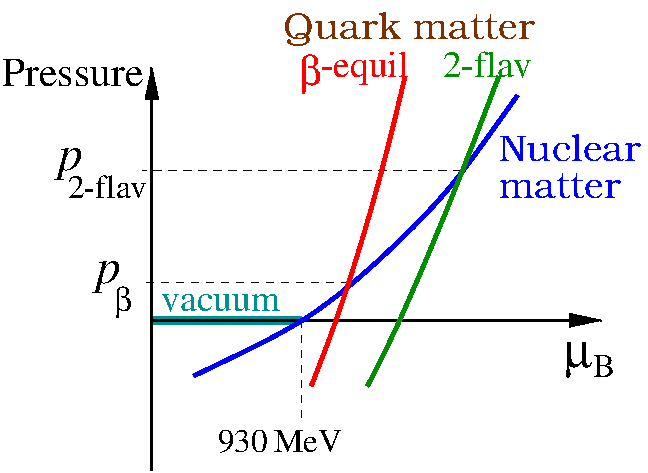
\includegraphics[width=0.65\columnwidth]{Plots/pressure_mu_pos.pdf}%
  \caption{Pressure comparison between phases at some arbitrary temperature. 
  %\mga{The ``2-flav'' line shows the baryon chemical potential of quark matter with exactly the same flavor content as nuclear matter at the same pressure.} 
  \mgacom{Maybe there shouldn't be a 2-flav line, since it's not an equilibrated phase with a definite composition at given $\mu_B$. We could just show the $P_\text{2-flav}$ dashed line.} Above pressure $P_\be$, 3-flavor chemically equilibrated quark matter is favored over nuclear matter. At $P>P_\text{2-flav}$, quark matter with the same flavor content as nuclear matter becomes favored, so weak interactions are no longer required for the conversion of nuclear to quark matter.
  } \label{fig:pressure-mu}
\end{figure}


\begin{figure}[t]
  \centering
  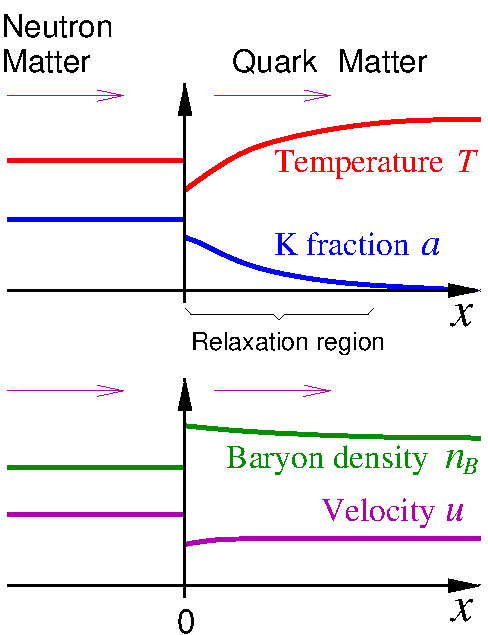
\includegraphics[width=0.65\columnwidth]{Plots/boundary_schematic.pdf}%
  \caption{
   Schematic illustration of the expected boundary profile. Note the discontinuities in some thermodynamic properties at the phase boundary located at $x=0$, followed by relaxation to beta equilibrium as $x\to\infty$. \mga{In the adiabatic case, temperature will also show a discontinuity at $x=0$ followed by relaxation to an asymptotic value as $x\to\infty$.}
  } \label{fig:boundary_schematic}
\end{figure}

\section{Formalism and assumptions}
\label{sec:formalism}

\subsection{Main assumptions}\label{sec:assumptions}

We assume the phase boundary is well approximated as a flat plane which can therefore be modeled as a one-dimensional system. This is a reasonable approximation for neutron star mergers, where the curvature of the boundary is on the kilometer scale, while its thickness is of order micrometers \mga{(see Eq.~\eqref{eq:conversion-thickness})}.
We defer any discussion of instabilities that would lead to a more complicated front geometry.
 \AHcom{As far as I know, people assume that instabilities work on the cm scale, which would still give us many orders of magnitude compared to micrometer. So the planar assumption should be fairly solid}
We assume that the surface tension of the phase boundary is large enough that mixed phases are not favored. We model the nuclear phase as pure neutron matter described by the QMC-RMF3 mean field theory~\cite{Alford:2022bpp,Alford:2023rgp,qmc_rmf3}. We model quark matter as a Fermi gas of massless noninteracting up, down, and strange quarks~\cite{Chodos:1974je,Farhi:1984qu}.

\mga{We will assume that the phase boundary is at a pressure where, in the range of temperatures relevant to neutron stars, 3-flavor beta-equilibrated quark matter is favored over nuclear matter (approximated as neutron matter in our case), but 2-flavor quark matter with the same flavor content as nuclear matter is not favored. I.e., the ambient pressure $P$ is between $P_\be$ and $P_{\text{2-flav}}$ in Fig.~\ref{fig:pressure-mu}.  Thus weak interactions are required to complete the conversion of the metastable nuclear matter to quark matter. (In the adiabatic case the comparison is more complicated because the two phases are at different temperatures, see Sec.~\ref{sec:speed-adiabatic}).} \AHcom{So only because we model nuclear matter as neutron matter, the flavor content is exactly ud in ration 1:2, just like two-flavor charge neutral QM. But chemically equilibrated nuclear matter and two-flavor QM will have a different flavor content, and this will probably lead to an even slower speed because we now need Urca. I think this should be discussed?} \mgacom{What matters is whether quark matter with exactly the flavor content of neutron matter is favored. Such quark matter won't be beta equilibrated.}
We will follow the standard approach to nuclear to quark conversion \cite{Olinto:1986je,Bombaci:2000cv,Bhattacharyya:2006vy,Niebergal:2010ds,Furusawa:2015vfn,Rosero-Gil:2020caj}
which exploits the clear separation between strong-interaction-driven processes such as local thermal equilibration and deconfinement, which can be treated as instantaneous on the time scales relevant to neutron star mergers, and flavor equilibration, which occurs via weak interactions and is therefore much slower and must be treated explicitly. 

We focus on the fastest flavor equilibration channel, the nonleptonic process
\begin{equation}
    d\ u \leftrightarrow u\ s\ .
\label{eq:nonleptonic}
\end{equation}
This equilibrates the quantum number that we will call ``K'', which measures the imbalance between down and strange quarks. 
We ignore electromagnetism, electrons, and neutrinos. We therefore neglect Urca processes, which are generally slower than the non-leptonic process \cite{Alford:2006gy,Alford:2025tbp,Sad:2007afd}, so their inclusion will make the boundary speed even lower.

As noted above, we assume local thermal equilibration is fast enough so that each fluid element has a well-defined temperature $T$. 
We will first write down the hydrodynamic equations that describe the movement of the fluid, including \mga{relativistic corrections,}\old{radiative loss} \mgacom{Not in the hydro eqns any more}
and diffusion of flavor (the $K$ quantum number) and heat.
In the body of the paper, however, we will \mga{self-consistently neglect relativistic hydrodynamic corrections since we will find that the boundary moves at speeds far less than the speed of light. Moreover, we will}
not explicitly treat the radiation or diffusion of heat via thermal conduction. Instead, we will calculate the boundary
propagation speed for two extreme cases: isothermal (the whole system is thermally equilibrated to the same temperature) and adiabatic (no thermal conduction).

\subsection{Formalism}

To calculate the speed at which the nuclear/quark phase boundary propagates through neutron matter, we will look for a steady state solution to the equations that describe the propagation of a deflagration front. 

We work in the rest frame of the phase boundary, which is located at $x=0$,
as illustrated schematically in Fig.~\ref{fig:boundary_schematic}.
At $x<0$ there is pure neutron matter which we take to be homogeneous, neglecting any disturbance propagating ahead of the phase boundary. The neutron matter flows towards the boundary with a velocity $u(x=0^-)$, which we aim to calculate. Matter at $x=0^-$ immediately deconfines into denser quark matter at $x=0^+$ with enough strangeness to be created from neutron matter \mga{under the prevailing conditions}  \mgacom{These weasel words are meant to cover the isothermal vs adiabatic vs everything in between}.
%(In the example shown in Fig.~\ref{fig:boundary_schematic} this is an endothermic reaction, so the temperature of freshly created quark matter at $x=0^+$ is less than in the neutron matter arriving at $x=0^-$.)  
\AHcom{I don't understand the enough strangeness part?}
\mgacom{If the quark matter doesn't have enough strangeness then it won't be energetically favored (extreme case: udd matter).}

At $x>0$ there is a conversion region where strange quarks are created via the weak interaction, leading to a flavor gradient that drives diffusion of strange quarks 
upstream towards the boundary. This is how the freshly created quark matter at $x=0^+$ can immediately have a larger strangeness fraction than was present in the incoming neutron matter. As $x\to\infty$ the quark matter approaches a fully beta-equilibrated state.

The parameters that describe the state of the matter at any given position $x$ are: 
%
\begin{equation}
\begin{array}{l@{\quad}l}
  n_B  & \text{baryon number density} \\
  n_K \equiv \dfrac{n_d-n_s}{2} & \text{``K'' density} \\
  u & \text{velocity in the $x$ direction} \\[0.5ex]
  T & \text{temperature} 
\end{array}
\label{eq:properties}
\end{equation}
%
From these one can, via the nuclear and quark equations of state (see Appendix~\ref{sec:bag_model}), calculate other properties such as pressure $P$, baryon chemical potential $\mu_B$, energy density, and the K chemical potential 
\begin{equation}
    \mu_K=\mu_d-\mu_s \ ,
\end{equation}
which relaxes towards zero via the weak interaction
\eqref{eq:nonleptonic}.

We will find it useful to define the local K fraction
\begin{equation}
 a(x)\equiv\frac{n_K(x)}{n_B(x)}\ .
 \label{eq:a_definition}
\end{equation}

\subsection{Hydrodynamic equations}
\label{sec:hydro-thermal}

%\AHcom{what would a dissipative correction look like as this would also be a result of the same weak interactions I think? du us BV is resonant at very low temperatures}\LBcom{I think $P \to P+\Pi$ is how it enters $T^{\mu \nu}$?}\\

Although our calculations will focus on the isothermal and adiabatic regimes, we first present the more general hydrodynamic equations including the effects of 
flavor and heat diffusion and radiative energy loss but neglecting viscous stresses. 

The stress-energy tensor without viscosity terms takes the form~\cite{Eckart:1940te,Harutyunyan:2023nvt}
\begin{equation}
T^{\mu\nu}=(P+\eps) U^\mu U^\nu-P g^{\mu\nu}\\
\JS{+U^\mu q_{\rm th}^\nu+q_{\rm th}^\mu U^\nu}\,,
\label{eq:stress_tensor}
\end{equation}
and the fluid flow is defined by the baryon current
\begin{equation}
    J_B^\mu=n_B U^\mu \,,
\end{equation}
where $U^\mu = (\gamma,u_x,u_y,u_z)$ is the baryon fluid four-velocity, \LB{with Lorentz factor $\gamma=1/\sqrt{1-v^2}$, spatial component of the four-velocity $u=\gamma v$, and lab-frame three-velocity $v$,}
%three velocity $v$ is the fluid velocity with  that frame is related with $u$ and Lorentz factor $\gamma$ by $u=\gamma v$ and  $\gamma=1/\sqrt{1-v^2}$,  %\mgacom{This sounds weird: relativistic expressions should be valid in any inertial frame.}
%\LB{The fluid 4-velocity is defined such that in the fluid rest frame, the flow of baryon number vanishes \mgacom{Seems obvious: do we need to say it?}\LBcom{Maybe we should say something about being in the rest frame of the boundary here.}}\mgacom{That's done a few lines below.}
and \LB{$q_{\text{th}}^\nu$ is the heat current which is purely spatial in the local fluid frame, i.e., $U_\mu q_{\text{th}}^\mu=0$.}
%\LBcom{?} \mgacom{I don't get this either}
%, satisfying $U_\mu q_{\text{th}}^\mu=0$.\LBcom{note move stuff from app A here}

\mga{We now apply the relevant conservation laws.}
Baryon number is conserved, while radiation can carry energy and momentum out of the fluid:
\mgacom{If we are going to neglect radiation in eq (16), is there any point in keeping it here?}\LBcom{I am fine without $Q^\nu$. Alex wanted this in the past so lets ask him.}
\begin{equation}
\begin{aligned}
    \partial_\mu J_B^\mu&=0 \, ,\\
    \partial_\mu T^{\mu\nu}&=\JS{-Q^\nu} \, .
\end{aligned}
\label{eq:formal-eqs}
\end{equation}
Here $Q^\nu$ is the radiation energy-momentum loss per unit spacetime volume. There is also a K quantum number current, whose conservation is violated by weak interactions,
\begin{equation}
    \partial_\mu J_K^\mu = -\Gamma_K\ ,
\end{equation}
where $\Gamma_K$ is the rate of down-to-strange quark conversion (see Appendix~\ref{sec:K-creation}) and 
\begin{equation}
    J_K^\mu = n_K U^\mu + D_K^\mu\ ,
\end{equation}
\begin{equation}
D_K^\mu
=
D_K\Delta^{\mu\nu}\partial_\nu n_K\ ,
\end{equation}
where $\Delta^{\mu \nu}=(g^{\mu\nu}-U^\mu U^\nu)$ projects onto directions orthogonal to the fluid four-velocity and $D_K$ is the K-diffusion coefficient.


We now formulate these conservation equations in the planar
phase boundary rest frame. Derivatives with respect to $t$, $y$, and $z$ vanish. Then baryon number conservation gives
\begin{equation}
\frac{d}{dx}(n_Bu)=0\,,
\end{equation}
and energy-momentum conservation reduces to 
\begin{align}
\frac{d}{dx}\left[(P+\eps)\gamma u+\frac{\gamma^2+u^2}{\gamma} q_{\rm th}^x\right]&=-Q^0\,,\label{eq:energy_balance_exact}\\
\frac{d}{dx}\left[(P+\eps)u^2 + P +2u q_{\rm th}^x\right]&=-Q^x\,.\label{eq:momentum_balance_exact}
\end{align}
Note that we have used $q_\mu U^\mu=0$ and $\gamma^2 - u^2 = 1$.
%For the slow conversion fronts considered here with $Q^\nu=0$, constant pressure is accurate up to $O(u^2)$ corrections, as shown in Appendix~\ref{sec:heat_transport}.

For the heat current $q^\mu_{\rm th}$ we use the Eckart heat law \LB{ neglecting an acceleration term.}~\cite{Eckart:1940te,Lopez-Monsalvo:2010oeo} 
\begin{equation}
q_{\rm th}^{x}=-\kappa_{\rm th}\gamma^2\frac{dT}{dx} \,,
\label{eq:heat_flux_main}
\end{equation}
where $\kappa_{\rm th}$ is the thermal conductivity~\cite{Heiselberg:1993cr}.

In our 1-dimensional geometry
we write the spatial component of the K current as
\begin{equation}
    J_K^x = un_K - \gamma^2 D_K\frac{d}{dx}n_K \ .
\end{equation} 
See Appendix~\ref{sec:K-diffusion} for our approach to estimating the diffusion coefficient $D_K$.

\mga{Since we neglect neutrinos, which are the main channel for radiative energy loss, we set} $Q^\mu=0$ to
arrive at the following set of hydrodynamic equations
%
\begin{subequations}\label{eq:front_system_thermal}
\begin{align}
\frac{d}{dx}(u n_B)&= 0\,, 
\label{eq:baryon_conservation_thermal}\\
\frac{d}{dx}\left[(P+\eps)\gamma u+\frac{\gamma^2+u^2}{\gamma} q_{\rm th}^x\right]&=0\,,
\label{eq:energy_conservation_thermal}\\
\frac{d}{dx}\left[(P+\eps)u^2 + P +2u q_{\rm th}^x\right]&=0\,,
\label{eq:momentum_conservation_thermal}\\
\frac{d}{dx}J_K &= -\Gamma_K\,.
\label{eq:K_conservation_thermal}
\end{align}
\end{subequations}
In the following sections we will solve 
Eqns.~\ref{eq:front_system_thermal}
to obtain the propagation speed of the phase boundary $u$ in the isothermal and adiabatic limits. 

The isothermal limit (Sec.~\ref{sec:speed-isothermal}) is obtained by assuming infinite thermal conductivity, so the system will have a uniform temperature.

The adiabatic limit Sec.~\ref{sec:speed-adiabatic}) is obtained by setting the thermal conductivity to zero, so entropy is conserved, apart from
contributions from the weak interactions that
relax the system towards beta-equilibrium \LBcom{and flavor diffusion?} \mgacom{Diffusion moves K-ness around but it's the weak interactions that create the K-ness that's needed to equilibrate the quark matter}.
The steady-state boundary profile will then have a spatially varying temperature.
%For $\kappa_{\rm th}=0$ and $Q_\nu=0$, Eq.~\eqref{eq:energy_conservation_thermal} instead gives $d[(P+\eps)u\gamma]/dx=0$, the adiabatic case of Sec.~\ref{sec:speed-adiabatic}.

Anticipating the results that will be presented in Sec.~\ref{sec:results}, which find that the typical boundary propagation speeds are
around a millionth of the speed of light, we will ignore relativistic effects from now on by setting $\gamma = 1$ and dropping $\mathcal{O}(u^2)$ corrections, so we no longer distinguish the three-velocity $v$ from the $x$ component $u=\gamma v$ of the four-velocity.\LBcom{Which equations are actually used when solving for the boundary speed numerically?}

\section{Boundary propagation speed: isothermal case}
\label{sec:speed-isothermal}

%We now describe how to calculate $u(0^-)$, the speed at which the nuclear/quark phase boundary propagates through neutron matter, in the limit where there is a single uniform temperature across both phases.

\subsection{Isothermal hydrodynamic equations}
\label{sec:isothermal-equations}


The isothermal limit is obtained by taking
$\kappa_{\rm th}\to\infty$ in Eqns.~\ref{eq:front_system_thermal}.
This yields\LBcom{are we actually solving eqs 17?}
\begin{subequations}\label{eq:front_system_isothermal}
\begin{align}
\frac{d}{dx}(u n_B)&= 0\,, 
\label{eq:baryon_conservation_isothermal}\\
\frac{d}{dx}T(x) &=0\,,
\label{eq:isothermal_condition}\\
\frac{d}{dx} P(x) &=0\,,
 \label{eq:momentum_conservation_isothermal}\\
 \frac{d}{dx}J_K &= -\Gamma_K\ ,
    \label{eq:K_conservation_isothermal}
\end{align}
\end{subequations}
\mga{where we obtained Eq.~\eqref{eq:isothermal_condition} from the $\kappa_{\rm th}\to\infty$ limit of Eqs.~\eqref{eq:energy_conservation_thermal} (or 
\eqref{eq:momentum_conservation_thermal}) combined with \eqref{eq:heat_flux_main}. Eq.~\eqref{eq:momentum_conservation_isothermal} is obtained by writing
Eqs.~\eqref{eq:energy_conservation_thermal} and
\eqref{eq:momentum_conservation_thermal}) as $(P+\eps)u + q_\text{th} = C_1$ and $P+2uq_\text{th}=C_2$ where $C_1$ and $C_2$ are independent of $x$, and
eliminating $q_\text{th}$ and dropping terms of order $u^2$ to obtain $P = C_2 - 2uC_1$. Using the fact that $q_\text{th}\to 0$ at $x\to\infty$ (because all gradients including $dT/dx$ vanish) we can see that $C_1/C_2$ is of order $u$, so again dropping terms of order $u^2$ we find that $P$ is independent of $x$.}

%
The first three equations give us simple constancy conditions for the baryon current, temperature, and pressure.
%\begin{equation}
%\left.
%\begin{array}{rl}
% J_B &=n_Bu \,, \\[1ex]
% \Pi &=P \,,\\[1ex]
% T
%\end{array}
%\right\}\parbox{6em}{independent of %$x$.}
%\label{eq:conserved_fluxes}
%\end{equation}
%
Thus to obtain the profile of the moving phase boundary we only need to solve the K flux equation Eq.~\eqref{eq:K_conservation_isothermal}, a second-order differential equation that can be recast as two first-order differential equations for the K density and current,
\begin{subequations}
\label{eq:reduced_BVP}
\begin{align}
 \frac{d}{dx}n_K &=\frac{un_K-J_K}{D_K}\,,
\label{eq:BVP_nK}\\
 \frac{d}{dx}J_K &=-\Gamma_K\,.
\label{eq:BVP_jK}
\end{align}
\end{subequations}
%
where $D_K$ and $\Ga_K$ in quark matter ($x>0$) are given in Appendices \ref{sec:K-diffusion} and \ref{sec:K-creation}. We do not need to know $D_K$ or $\Ga_K$  in nuclear matter ($x<0$), because we assume it is uniform and equilibrated. At the boundary itself we expect $\Ga_K$ will remain finite, but the right side of Eq.~\eqref{eq:BVP_nK} will include a 
delta-function singularity (as the corresponding equation for $dn_B/dx$ does, since $u$ and $n_B$ both have discontinuities).


There is now a well defined procedure for constructing a solution to the hydrodynamical equations.  
Assume we have solved Eq.~\eqref{eq:reduced_BVP} up to some position $x$, giving $n_K(x)$ and $J_K(x)$.
We can combine this with the already-specified $x$-independent values of
$J_B$, $P$, and $T$
%the \eqref{eq:conserved_fluxes} 
and the quark matter equation of state (Appendix~\ref{sec:bag_model}) at the prescribed temperature to solve for the remaining properties of the matter at $x$, such as $n_B(x)$, $u(x)$, $\mu_B(x)$, $\mu_K(x)$, etc.
This allows us to calculate $D_K(x)$ and $\Gamma_K(x)$ (see Appendices~\ref{sec:K-creation} and \ref{sec:K-diffusion}) and thereby obtain $n_K(x+\de x)$ and $J_K(x+\de x)$.

\subsection{Boundary conditions}
\label{sec:boundary_conditions}

To construct the boundary profile we need 5 initial conditions  specifying the state of the incoming nuclear matter: $n_B(0^-)$, $n_K(0^-)$, $dn_K/dx(0^-)$, $T(0^-)$, $u(0^-)$.
However, since we assumed the incoming matter is  neutron matter, for which $n_K=n_d/2$, we have
\begin{equation}
  n_K(0^-)=n_B(0^-)\,,
  \label{eq:nK-nuclear}
\end{equation}
and since we have assumed the neutron matter is homogeneous,
\begin{equation}
  \dfrac{dn_K}{dx}(0^-)=0\,,
  \label{eq:dnKdx-nuclear}
\end{equation}
so we only need to specify $n_B(0^-)$,  $T(0^-)$, $u(0^-)$, which fixes the $x$-independent parameters $J_B$ and $P$ for the whole solution.

The first step in solving the equations is to relate the K density and current at $x=0^+$ to the initial conditions at $x=0^-$, after which we can evolve the solution to $x=+\infty$ using \eqref{eq:reduced_BVP}.

Integrating Eq.~\eqref{eq:BVP_jK} 
% Eqs.~\eqref{eq:reduced_BVP} 
across the sharp interface yields the continuity condition $J_K(0^+)=J_K(0^-)$, which can be re-expressed using Eq.~\eqref{eq:BVP_nK} as a
hydrodynamic jump condition,
\begin{equation}
 u(0^+)n_K(0^+)
 -\left[D_K\frac{dn_K}{dx}\right]_{0^+}
 =u(0^-)n_K(0^-)\,.
\label{eq:jump_K-}
\end{equation}
We do not need to know the K diffusion coefficient on the nuclear side because we have assumed there is no gradient there. 
%(or equivalently $a(0^+)$) 
%Eq.~\eqref{eq:jump_K-} fixes $dn_K/dx(0^+)$ in terms of $n_K(0^+)$ 

We cannot integrate Eq.~\eqref{eq:BVP_nK} to obtain an analogous relation between $n_K(0^+)$ and $n_K(0^-)$, because \mga{the right side of Eq.~\eqref{eq:BVP_nK} includes an unknown delta-function divergence at $x=0$.}
We therefore have to treat $n_K(0^+)$ as an additional parameter of the system.
In our calculations we will choose the value of $n_K(0^+)$ that maximizes the speed of the boundary.

Since the solution must yield equilibrated quark matter as $x\to\infty$, we also impose the boundary condition 
\begin{equation}
    \mu_K(\infty)=0 \ ,
\end{equation}
which for our model of quark matter is equivalent to $n_K(\infty)=0$.
This turns \eqref{eq:reduced_BVP} into an eigenvalue problem, where for given $n_B(0^-)$, $T(0^-)$, and $n_K(0^+)$ there is only one value of the incoming neutron matter velocity $u(0^-)$ that yields a valid solution.


\mga{
The final step is to choose a value for $n_K(0^+)$, or equivalently (see Eq.~\ref{eq:a_definition})
$a(0^+)$, the K fraction in freshly created quark matter. This lies between 0 (corresponding to quark matter with equal numbers of $u$, $d$, and $s$ quarks), and $1$ (corresponding to quark matter with no strangeness, i.e., having the same flavor content as neutron matter, $a(0^-)=1$).  We will  choose it so as to give the maximum speed of the boundary. We expect that the speed will be a monotonically increasing function of $a(0^+)$, since
neutron$\to$quark matter conversion becomes easier (requires fewer weak interactions and less K diffusion) as the flavor content of the quark matter becomes more similar to that of nuclear matter. This expectation will be confirmed by our analytic approximation (Appendix~\ref{sec:isothermal-analytic}).
 
We will therefore set $a(0^+)$ to $A_{\text{iso}}$, the largest physically possible value of $a(0^+)$, which is given by saturating the requirement that the quark matter at $x=0^+$ must be thermodynamically favored over the neutron matter at $x=0^-$. Since these two forms of matter are at the same pressure and temperature, neutron$\to$quark conversion is favored when
the average chemical potential of 3 quarks in freshly created quark matter,
$\mu^\text{avg}(0^+)=\mu_B(0^+) + n_K(0^+)\mu_K(0^+)/n_B(0^+)$
is lower than the average chemical potential of a neutron in the
incoming neutron matter, $\mu^\text{avg}(0^+)=\mu_B$. Thus $A_{\rm iso}$ is specified as the value of $a(0^+)$ for which the average chemical potentials are equal. It is determined by the equation of state, see Eq.~\eqref{eq:a0plus_max}.
Quark matter with $a(0^+)>A_{\rm iso}$ would have insufficient strangeness to make it favored over neutron matter (see Fig.~\ref{fig:pressure-mu} and Ref.~\cite{Alford:2014jha}).
}

We can now obtain the boundary speed in terms of the density and temperature of the neutron matter.
%and the K fraction in the freshly created quark matter.
We do this by solving \eqref{eq:reduced_BVP} as described in Sec.~\ref{sec:isothermal-equations} using the boundary conditions described above.

Our results presented in Sec.~\ref{sec:results} will be obtained by solving the differential equations numerically.
%, as described in Appendix~\ref{sec:numerical}.
However, as we now describe, one can also formulate an approximate analytic solution, which is helpful for interpreting the results.

\subsection{Analytic approximation}
\label{isothermal-approx}

\mga{In the conversion region the matter follows an isobar in the $(\mu_B,\mu_K)$ plane. Since $\mu_K$ is typically much smaller than $\mu_B$ the dominant contribution to the pressure is of order $\mu_B^4$ (Eq.~\eqref{eq:QM-EoS-2nd-order}) so
$\mu_B$ is expected to vary only slightly. This is confirmed by plotting a typical conversion region profile in the $(\mu_B,\mu_K)$ plane (red line in Fig.~\ref{fig:isobar_muB_muK}). This motivates an approximation where $\mu_B$ and $n_B$ (and therefore the velocity $u$, see \eqref{eq:baryon_conservation_isothermal}) are assumed independent of $x$, taking constant values $\mu_B^{(+)}$, $n_B^{(+)}$ , and $u^{(+)}$ over the region $x>0$. The result,  derived in Appendix~\ref{sec:isothermal-analytic}, is an approximate expression for the maximum iosthermal boundary speed,}
\begin{equation}
\begin{aligned}
u^{\max}_{\rm iso}(0^-)\simeq&(98\, {\rm m/s})
\frac{n_B^{(+)}}{n_B(0^-)}\\
&\times\left(\frac{\mu_B^{(+)}}{1200\,\MeV}\right)^\frac{17}{6}
\left(\frac{10\,\MeV}{T}\right)^\frac{5}{6}\\
&\times\frac{A_{\rm iso}\sqrt{A_{\rm iso}^2+162\pi^2T^2/(\mu_B^{(+)})^2}}
{\alpha_s^{5/6}\sqrt{1-A_{\rm iso}}\sqrt{1+\xi A_{\rm iso}}}\ .
\end{aligned}
\label{eq:isothermal_speed_scaling}
\end{equation}
%
where $A_\text{iso}$ is given by 
Eq.~\eqref{eq:a0plus_max} and $\xi$ is the sharpness factor (Appendix~\ref{sec:xi-shape}) characterizing the profile of the conversion region. 

\begin{figure}
    \centering
    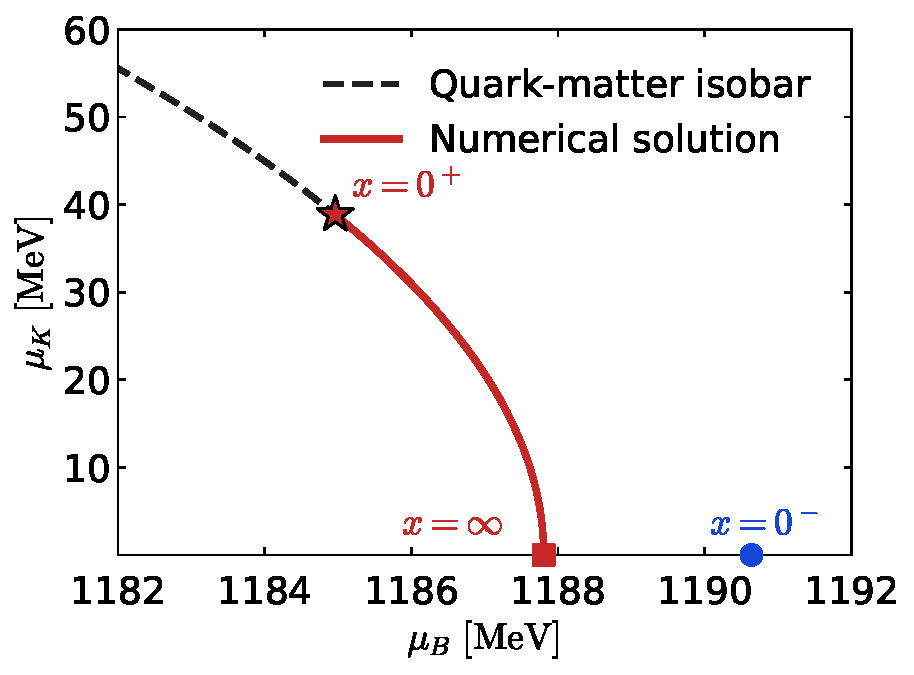
\includegraphics[width=\linewidth]{Plots/isothermal_muB_muK_plane.pdf}
    \caption{Constant-pressure trajectory through the quark conversion layer in the $(\mu_B,\mu_K)$ plane at fixed $T=10\,\MeV$.
    The red curve is the quark-matter isobar for $n_B(0^-)=3n_0$ and $B^{1/4}=189.1566\,\MeV$.
    The red arrows run from the just-deconfined state at $x=0^+$ to the equilibrated state at $x\to\infty$; the green arrow represents deconfinement from the nuclear-side marker at $x=0^-$. \LBcom{move x labels down a little so plot markers are not covering the numbers}
    }
    \label{fig:isobar_muB_muK}
\end{figure}

We can also estimate the thickness $L_{\text{conv}}$ of the conversion region, which determines the range of curvature that is compatible with our assumption of a planar geometry.
If the boundary moves slowly then when $a \ll 9\pi T/\mu_B^{(+)}$, which is guaranteed to occur at large $x$ where $a\to 0$, the K current equation reduces to
\begin{equation}
    \dfrac{d^2 a}{dx^2} =
    \dfrac{\ga_K}{D_K}\biggl(\dfrac{9\pi T}{\mu_B^{(+)}}\biggr)^{\!2} a \,.
\end{equation}
At large $x$ the temperature reaches an asymptotic value $T(\infty)$ (equal to $T$ in the isothermal case), so we can estimate the thickness of the conversion region as
\begin{align}
    L_{\text{conv}} &\approx \dfrac{\mu_B^{(+)}}{9\pi T(\infty)}\sqrt{\dfrac{D_K}{\ga_K}} \notag\\
    &= (0.2\,\mu\m)\,\dfrac{1}{\al_s^{5/6}}
    \biggl(\dfrac{1200\,\MeV}{\mu_B^{(+)}}\biggr)^{\!7/6}
     \biggl(\dfrac{10\,\MeV}{T(\infty)}\biggr)^{\!11/6}
    \,, \label{eq:conversion-thickness}
\end{align}
where we evaluated $D_K$ using \eqref{eq:diffusion_coefficient} with $T=T(\infty)$ and $\gamma_K$ from Eq.~\eqref{eq:cubic_rate}.
This supports our use of the planar approximation, since the typical curvature of a quark/nuclear boundary in neutron stars will be of order kilometers, much larger than the thickness of the boundary.

\section{Boundary propagation speed: adiabatic case}
\label{sec:speed-adiabatic}


\subsection{Adiabatic hydrodynamic equations}
\label{sec:adiabatic-equations}

\mga{The adiabatic limit is obtained by}
setting thermal conductivity $\kappa_{\rm th}=0$ and radiative energy loss $Q_\nu=0$ in Eq.~\eqref{eq:front_system_thermal}.
\mga{Dropping terms of order $u^2$ we obtain} the adiabatic steady-state  equations \JScom{the numerical code still includes full relativistic corrections, }
%
\begin{subequations}\label{eq:front_system_adiabatic}
\begin{align}
\frac{d}{dx}(u n_B)&= 0\,,
\label{eq:baryon_conservation}\\
\frac{d}{dx}(h u) &=0\,,
\label{eq:energy_conservation}\\
 \frac{d}{dx}(\old{h u^2+}P)&=0\,,
 \label{eq:momentum_conservation}\\
 \frac{d}{dx}J_K &= -\Gamma_K\ .
    \label{eq:K_conservation}
\end{align}
\end{subequations}
%
where $h=P+\eps$ is the enthalpy.
The first three equations impose constant baryon flux, enthalpy flux and pressure.
%\begin{equation}
% E=hu\,.
% \label{eq:energy_flux_adiabatic}
%\end{equation}
%\mgacom{Do we need to define $E$? Do we use it anywhere?}
These fluxes are fixed by choosing the baryon density, temperature, and speed of the incoming nuclear matter, $(n_B(0^-)$, $T(0^-)$, and $u(0^-)$.  Eq.~\eqref{eq:K_conservation} leads to the same K transport equations as in the isothermal case \eqref{eq:reduced_BVP}, with the same boundary conditions  (Sec.~\ref{sec:boundary_conditions}). As before, there is only one value of the boundary speed $u(0^-)$ that yields a well-behaved solution to the equations.
The difference is that in the evolution procedure described in Sec.~\ref{sec:isothermal-equations} we now determine $T(x)$ from the constant enthalpy flux. 

\mga{
As in the isothermal case, we set the K density of freshly created quark matter $\azp$ to the largest physically possible value, because that gives the fastest boundary speed. This corresponds to setting the temperature of freshly created quark matter $T(0^+)$ to zero.
Intuitively this makes sense: larger values of $\azp$ correspond to quark matter with flavor content that is as similar as possible to neutron matter for which $a=1$. But as $\azp$ grows the quark matter has more unequal populations of the three flavors, making it less energetically favored. As $\azp$ becomes larger, the creation of the quark matter becomes more endothermic, until we reach the extreme case where the freshly created quark matter has zero temperature.

This picture is confirmed by our numerical calculations. The red line in Fig.~\ref{fig:isobar_a_T} shows the projection of a solution to the adiabatic steady state equations onto the $(a,T)$ plane.
At $x=0^+$ the quark matter has some initial K fraction $a(0^+)$ which determines the initial temperature $T(0^+)$ (the red star in the figure).
As $x$ increases, the system moves upwards along the red line, ending at $a=0$ and some final temperature $T(\infty)$ when $x\to\infty$ (the red square in the figure). 
%We see from the figure that the analytical approximation (dashed line) gives a reasonably accurate approximation to the actual path followed in the $(a,T)$ plane.
We define $A_\text{adb}$ as the maximum possible value of $a(0^+)$, which is achieved if $T(0^+)=0$. 

In our numerical computations presented in Sec.~\ref{sec:results}) we will set $T(0^+)$
to a small but finite value, for numerical tractability.


\begin{figure}[t]
  \centering
  \IfFileExists{Plots/T_a_constant_pressure.pdf}{%
    \includegraphics[width=\columnwidth]{Plots/T_a_constant_pressure.pdf}%
  }{%
    \includegraphics[width=\columnwidth]{Hydrodynamical combustion/Plots/T_a_constant_pressure.pdf}%
  }
  \caption{Constant-pressure trajectory through the quark conversion layer \mga{in the adiabatic case, for $T(0^-)=10~\MeV$, $B^{1/4}=180~\MeV$, $n_B(0^-)=3n_0$, and $a(0^+)=0.55$.
  The red curve is from the profile obtained by numerically solving the K flux equation.}  The dashed curve is the quarter ellipse from the analytic approximation  Eq.~\eqref{eq:constant_pressure_path}.
      }
\label{fig:isobar_a_T}
\end{figure}

\subsection{Analytic approximation}
\label{sec:adiabatic-approx}

As in the isothermal case, we can obtain an approximate analytic expression for the  propagation speed of the boundary by assuming that as well as the conserved fluxes mentioned above, baryon density $n_B^{(+)}$,
baryon chemical potential $\mu_B^{(+)}$, and fluid speed $u^{(+)}$ are independent of $x$ in the quark matter region. Temperature and K fraction $a$ are allowed to vary with $x$. 
The calculation is described in Appendix~\ref{sec:adiabatic-analytic}, and yields the result (Eq.~\eqref{eq:adiabatic_approx_appendix})}
%
\begin{align}
u^{\max}_{\rm adb} (0^-) = (82\,\m\s^{-1})\,
&\dfrac{n_B^{(+)}}{n_B(0^-)}
\biggl(\!\dfrac{\mu_B^{(+)}}{1200\,\MeV}\!\biggr)^{\!2}
\times \notag\\
& \dfrac{ A_{\rm adb}^{7/6}}{\al_s^{5/6} \sqrt{1-A_{\rm adb}}\sqrt{1+\xi A_{\rm adb}}} \, .\label{eq:adiabatic_speed_scaling}
\end{align}
where $A_\text{adb}$ is determined by the quark matter equation of state, and is given in Eq.~\eqref{eq:a-max}.
Thus the typical speed of the boundary is expected to be of order $100\m\,\s^{-1}$.
\mga{In Sec.~\ref{sec:results} we will see that this agrees well with the numerical solution at lower temperatures and densities.}
In this expression the only factor that could drive the speed to a significantly higher value is $1/\sqrt{1-A_{\rm adb}}$.
To see when $A_{\rm adb}$ could approach 1 we recall that $A_{\rm adb}$ is the largest possible K fraction in the freshly created quark matter at $x=0^+$.
The K fraction in neutron matter is 1, so if $A_{\rm adb}=1$ then the pressure at the boundary is so high that that nuclear matter can convert to quark matter with the same flavor content.
In this case no weak interactions are needed, so it is not surprising that \mga{at such high pressures} our approach breaks down.




\section{Results}
\label{sec:results}

\JS{
Do we need to re-calculate and re-produce every plot? 
\begin{itemize}
    \item use quark EoS without gluons
    \mgacom{No, as long as we can cite reputable sources for the EoS with gluons}
    \item use full phase-space integral rate $\Gamma_K$ for full numerical calculations
    \mgacom{I don't think we decided on this}
    \item don't use relativistic corrections for both isothermal and adiabatic full numerical methods. 
    \item use $\alpha_s = 0.4$
\end{itemize}
}

\mga{We will calculate the maximum phase boundary propagation speed by numerically solving the steady state equations for the boundary profile, in the isothermal (Sec.~\ref{sec:isothermal-equations},\ref{sec:boundary_conditions})
%\eqref{eq:front_system_isothermal} 
and adiabatic  (Sec.~\ref{sec:adiabatic-equations})
%\eqref{eq:front_system_adiabatic} 
limits.

For the quark matter EoS, the only free parameter is the bag constant, which we set to $U_\text{bag}^{1/4}=189.2\,\MeV$, which 
places the zero-temperature nuclear-quark phase transition at density $n_B^{\rm crit}(T{=}0)=3n_0$.

}

\AHcom{I think if we have Fig1 as schematic, we should have an equivalent figure here with an actual result?}



\subsection{Isothermal case}

\mga{
In Figs.~\ref{fig:speed-isothermal-linear} and \ref{fig:speed-isothermal-log} we show contour plots of the numerically calculated maximum boundary propagation speed, as a function of the neutron matter density and the ambient temperature.
The white region is the range of densities and temperatures where the boundary propagates because neutron matter is metastable against conversion to quark matter with different flavor content, specifically, more strangeness. In the grey region at lower left, the ambient pressure is below the transition pressure so quark matter is not favored over neutron matter. As one would expect, the propagation speed drops to zero as the system approaches this regime.
In the grey region at upper right, the pressure is so high that quark matter with the same flavor content as neutron matter is thermodynamically favored ($P>P_\text{2-flav}$ in Fig.~\ref{fig:pressure-mu}) so boundary propagation can proceed without weak interactions. In our formalism the propagation speed diverges because $A_\text{adb}\to 1$ as one approaches that regime.

In Fig.~\ref{fig:speed-isothermal-linear} we see that the speed also appears to diverge at $T\to 0$ at fixed neutron matter density. To clarify this we also provide a log scale plot, Fig.~\ref{fig:speed-isothermal-log}, which shows shows the same numerically calculated data (solid lines and points) along with the values yielded by the analytic approximation Eq.~\eqref{eq:isothermal_speed_scaling}. Firstly, this confirms that the analytic approximation is reasonably accurate. Secondly, since the analytic approximation can be evaluated at low temperatures where the numerical method becomes difficult to implement, it allows us to see how low the temperature would have to be for the phase boundary to move appreciably on the distance and time scales relevant for mergers, supernovas, etc.
Finally, the analytic approximation shows us why the speed diverges at low temperature: it is because the K-diffusion coefficient (which is proportional to the mean free path) diverges at low temperature.  \mgacom{Talk about when this invalidates our approach as mfp gets comparable to the conversion region}

The main message of Figs.~\ref{fig:speed-isothermal-linear} and \ref{fig:speed-isothermal-log} is that under typical thermodynamic conditions of mergers and supernovas ($T\gtrsim 1,\MeV$) the phase boundary between metastable nuclear matter and quark matter will propagate at speeds of order 100 to $1000\,\m\s^{-1}$ at most. (Recall that in making approximations and parameter choices we favored those that led to faster speeds.) In mature single neutron stars, which have lower core temperatures, the boundary could move faster.
}

\begin{itemize}
  \item about contour plot: 
  \begin{itemize}
    \item existence of stable neutron matter region, and why it takes that shape
    \item $A_{\rm adb}>1$ region and why that shape
    \item velocity in between, also mention it diverge as the input goes close to $A_{\rm adb}=1$
  \end{itemize}
\end{itemize}



\begin{figure}
    \centering
    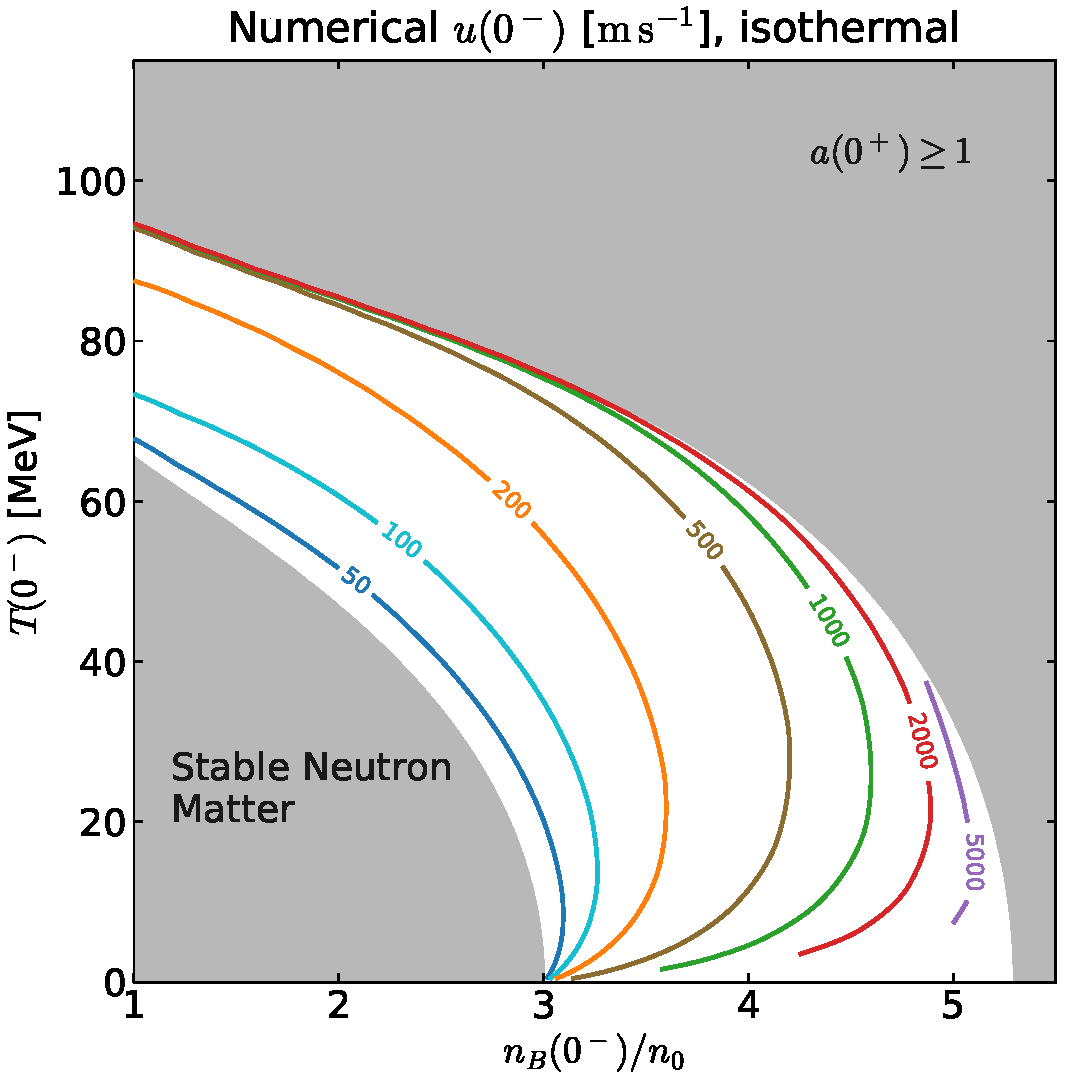
\includegraphics[width=\linewidth]{Hydrodynamical combustion/Plots/isothermal-numerical-contour.pdf}
    \caption{Contour plot of the numerically calculated maximum isothermal boundary propagation speed as a function of neutron matter density and ambient temperature.}
    \label{fig:speed-isothermal-linear}
\end{figure}

\begin{figure}
    \centering
    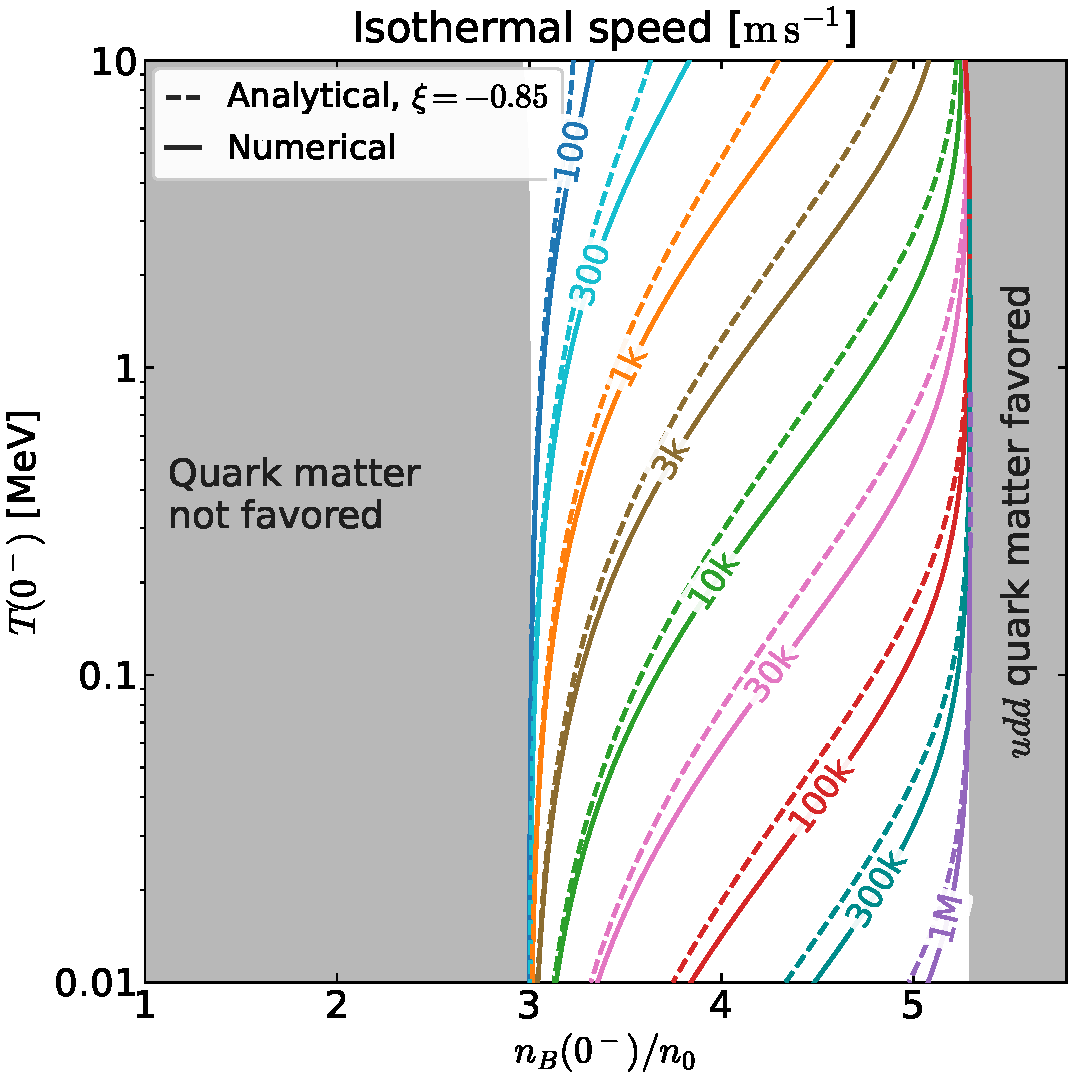
\includegraphics[width=\linewidth]{Hydrodynamical combustion/Plots/isothermal-analytic-numerical-logT.pdf}
    \caption{Contour plot of the maximum isothermal boundary propagation speed as a function of neutron matter density and ambient temperature. Solid lines and dots give the same numerically calculated values as are plotted in Fig.~\ref{fig:speed-isothermal-linear}. Dashed lines are the analytic approximation Eq.~\eqref{eq:isothermal_speed_scaling}.}
    \label{fig:speed-isothermal-log}
\end{figure}



\begin{figure}
  \centering
  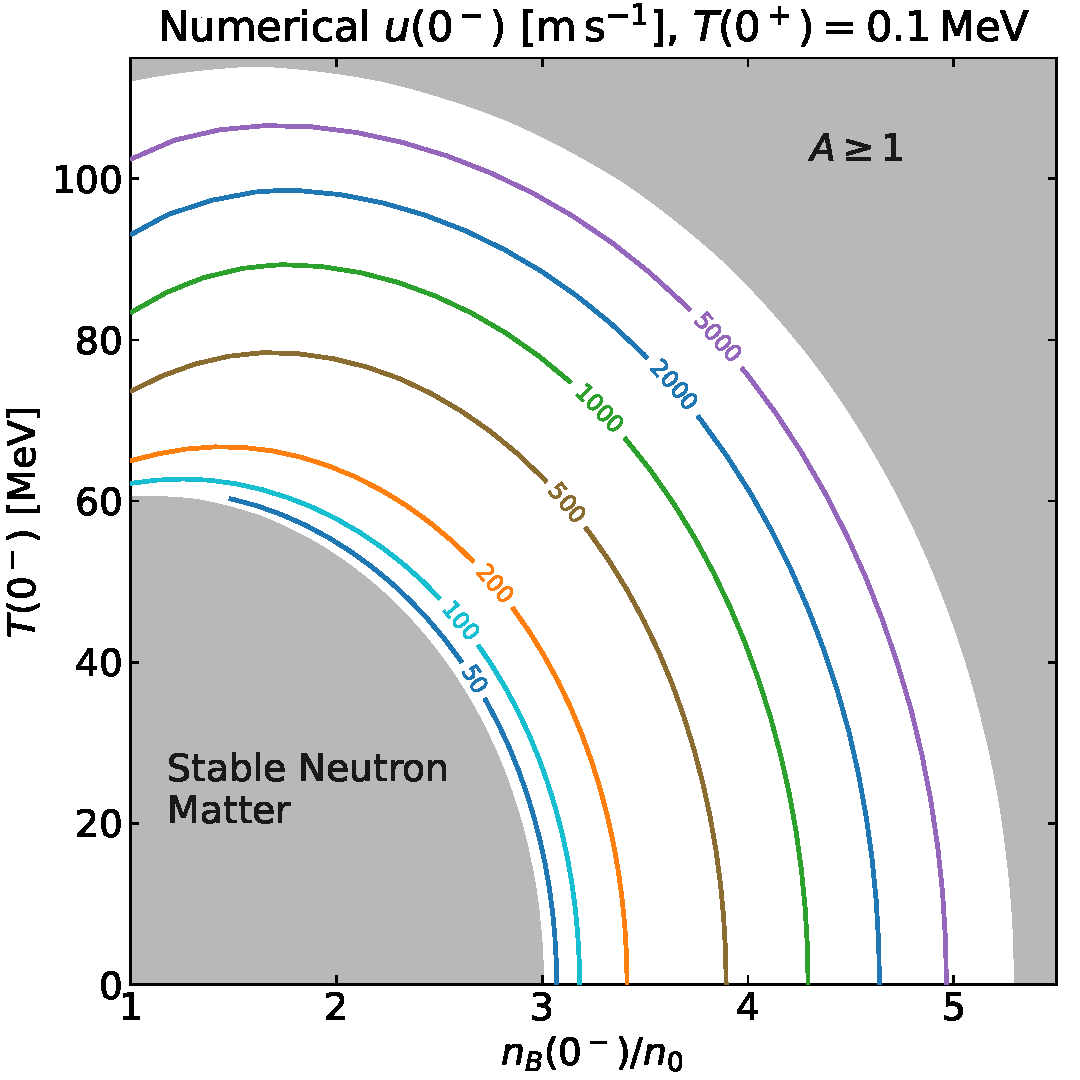
\includegraphics[width=\linewidth]{Plots/Numerical-contour.pdf}
  \caption{
  %\LBcom{In the isothermal case does the upper grey region curve back down at high T(0-)? I suspect not.}\JScom{No it doesn't}
  Full numerical phase-boundary speed $u(0^-)$ in $\m\,\s^{-1}$ as a function of the upstream baryon density and temperature, with $T(0^+)=0.1\,\MeV$ and $n_B^{\rm crit}(T{=}0)=3n_0\,.$
  The white band is the domain in which the moving-front solution exists.
  Below the lower boundary neutron matter is stable against the assumed conversion, while the region with $A_{\rm adb}\geq1$ lies outside the weak-interaction-limited branch described by our model.
  The contours are drawn at $50\,,$ $100\,,$ $200\,,$ $500\,,$ $1000\,,$ $2000\,,$ and $5000\,\m\,\s^{-1}\,.$}
  \label{fig:numerical}
  % Legacy aliases retained for collaborator notes later in the manuscript.
  \label{fig:u-analytical-loglog}
  \label{fig:T_vs_nB0-}
\end{figure}

\mgacom{Put this somewhere}
\mga{When we solve the profile equations numerically we will find that in the adiabatic case $\xi=-0.85$ is a good approximation (Appendix~\ref{sec:xi-shape}).}


\section{Conclusion}
\label{sec:conclusion}
\begin{itemize}
    \item Impact of instabilities, Urca processes, ... on phase boundary speed
\end{itemize}
\new{Our results allow us to speculate on the fate of interface modes in the inspiral.  Typical frequencies of interface modes depend on the EoS of nuclear and quark matter as well as the star's mass, where heavier stars show lower frequency resonances. The frequencies themselves range from a couple hundred to around $f=2000$ Hz (see Fig.~2 of Ref.~\cite{Counsell:2025hcv}). The existence and frequency of the interface mode furthermore critically depend on the conversion timescale, i.e.,~the speed with which the phase boundary between nuclear and quark matter can move via conversion of metastable nuclear matter to quark matter, or vice versa. If the phase boundary moves too fast, the restoring force for the interface mode and thus the mode itself vanish. All recent analyses \cite{Tonetto:2020bie,Counsell:2025hcv,Pereira:2025xsi}  set this velocity to zero and assume that on the millisecond timescale of the oscillation, the phase content is frozen. Depending on the energy absorbed by the mode, the amplitude ranges from a few millimeters to centimeters in the inspiral, and might reach several meters in the postmerger. Assuming a frequency of $f=700$ Hz, we can calculate the resonant velocity where the timescale of the oscillation matches the time given by the amplitude divided by the phase boundary velocity. In this resonant scenario, we expect viscous effects as described in \cite{Alford:2014jha} to become important, which can lead to an overdamping of modes \cite{Ghosh:2026ldg}. At even larger velocities, we expect the mode to lose its support (see discussion in the nuclear and hyperonic cases in Refs.~\cite{Zhao:2025pgx, Ghosh:2026ldg}) and vanish. In the inspiral, the resonant velocity ranges from $v_\text{res}=1$ m$/$s to $v_\text{res}=15$ m$/$s, which is within the range found in our calculation shown in Fig.~\ref{fig:u-analytical-loglog}. In the postmerger environment, the resonant velocity rises to $\mathcal{O}(1000\, \text{m/s})$, which is reached in the strongly metastable scenario (see Fig.~\ref{fig:T_vs_nB0-}). This shows that any accurate calculation of the interface mode must include the finite phase boundary velocity and viscous effects, potentially via the dynamical sound-speed formalism developed in Ref.~\cite{Zhao:2025pgx} and applied to quark matter in \com{cite Zhao Han Haber}.

Several recent works have studied the impact of a first-order phase transition on the postmerger, using model equations of state that include a nuclear/quark transition  \cite{Most:2018eaw,Bauswein:2018bma,Espino:2023llj,Weih:2019xvw,Harada:2023eyg,Bauswein:2020ggy,Haque:2022dsc,Fujimoto:2022xhv,Christian:2023hez,Fujimoto:2024ymt}. Features in the gravitational wave emission arise from the redistribution of mass as regions of the denser phase grow or shrink in response to pressure gradients in the violent collision between the stars.  We can now investigate how justified their used assumption of an instantaneous conversion of nuclear matter to quark matter is. A typical time step in a numerical relativity BNS simulation is $\Delta t\approx0.1\,\mu$s, and a typical spatial resolution is given by $\Delta x\approx 100$m. Any signal or phenomenon traveling at the speed of causality would need roughly $3\Delta t$ to traverse the entire fluid cell, which satisfies the Courant–Friedrichs–Lewy (CFL) condition \cite{Courant:1928lij} by design. Using the recent $6$ m resolution of Ref.~\cite{Kiuchi:2026pgb} with an estimated temporal resolution of $\Delta t \approx 10^{-8}$ s (corresponding to a CFL factor of $0.3$), a signal traveling at $c$ would require roughly $2\Delta t$ to traverse the fluid cell. Using a reasonable estimate of the fluid velocity from Fig.~\ref{fig:numerical} of $u(0^-)\approx500$ m/s, the phase boundary would take approximately $\tau_\text{cross}\approx12.5$ ms to cross the fluid cell, which corresponds to $1.25\times10^6\,\Delta t$.  This highlights that the assumption of instantaneous conversion has to be seen as an effective description. We thus need to compare the conversion timescale to the hydrodynamic timescales in the postmerger phase. Approximating the hydrodynamic merger timescale by the inverse of the dominant postmerger peak frequency of $f_\text{peak}\approx 2.5$ kHz yields $\tau_\text{hydro}\approx 0.4$ ms. 
We observe that the hydrodynamic timescale is significantly shorter than the evolution timescale of the quark matter phase, favoring a frozen composition approximation over an instantaneous conversion. However, in a long-lived remnant, the phase boundary would still be able to cross several fluid cells, indicating that a proper inclusion of the finite phase boundary velocity in merger simulations is required. 
}
\AHcom{this previous section might need an update number wise, I pulled the phase speed from the 0.1 MeV plot and we should use a hot plot}
\AH{
Given the estimates presented in the previous paragraphs, a more detailed calculation of the phase boundary velocity is needed.
\begin{itemize}[leftmargin=*]
    \item In this paper, we model the baryonic side as pure neutron matter. However, in compact stars, baryonic matter is composed of chemically equilibrated nuclear matter, which includes not only neutrons, but also protons, electrons, and muons in a composition determined by charge neutrality and chemical equilibration. Even hyperonic matter could be considered on the baryonic side of the phase boundary.
    \item The presence of leptonic particles opens up the possibility of proton or strangeness-changing Urca rates. The phase boundary velocity would then potentially be slowed down even further, as we now need to equilibrate multiple particle fractions on the quark matter side via the generally slower Urca processes. Our results thus likely present an upper bound on the velocity.
    \item At high temperatures, the physics of neutrinos might become important as neutrinos could cool down the conversion region, or if they get trapped, will alter the hydrodynamic description of the phase boundary. However, given our recent work in Refs.~\cite{Alford:2025jtm,Alford:2026kwd}, neutrino trapping on the microscopic scale of the phase boundary seems unfeasible, but could potentially play a role in the equilibrated baryonic or quark matter
    \item At the temperatures occurring in the inspiral, baryonic and quark matter might be found in a (color-)superconducting/superfluid state. Cooper pairing will not only alter the hydrodynamics of the problem, but suppresses the flavor-changing rates used in this work, and will also alter diffusive transport, thus furder slowing down the phase boundary.
    \item In this work, we have assumed that thermal equilibration across the phase boundary is happening on a timescale slower than the evolution of the phase boundary. Towards the end of the equilibration process, however, the phase boundary slows down (\AHcom{do we have a section explaining this?}. To not only reach flavor, but also thermal equilibration, thermal equilibration across the boundary has to be taken into account. Otherwise, the final state of the evolution will be wrongly described as a state where the baryonic and the quark matter phase stay at different temperatures.

    \item In this work, we assume that all profiles on the nuclear matter side are constant, and neglect any disturbance propagating ahead of the phase boundary. 
    \item Furthermore, the assumption of a steady state, which we deem reasonable, should be further investigated.
    \item Our hydrodynamic description is based on an ideal fluid description. Dissipative corrections might be taken into account in the stress-energy tensor, or be included via weak interactions as described in Ref.~\cite{Most:2022yhe}.
        \item If the phase boundary is driven by large-scale oscillations (as we expect it in the inspiral and the merger), the opposite scenario, where quark matter recombines to nuclear matter, has to be calculated. This will also allow us to estimate the strength of the so-called "phase conversion dissipation", a dissipative effect stemming from the out-of-phase movement of the actual phase boundary with the critical pressure \cite{Alford:2014jha}.
        \item Cooper pairing: influence on diffusion, weak interaction rates, anything else?
        \item surface tension?
\end{itemize}
}
\section*{Acknowledgements} We thank XXX (Nils Andersson? Suprovo Ghosh?) for valuable feedback and discussions.
MGA, LB, and AH are partly supported by the U.S. Department of Energy, Office of Science, Office of Nuclear Physics, under Award No.~\#DE-FG02-05ER41375. A.H.~furthermore acknowledges financial support by the UKRI under the Horizon Europe Guarantee project EP/Z000939/1.


\appendix
\section{Bag model of quark matter}
\label{sec:bag_model}

\mga{
Although we neglect electromagnetic interactions and leptons, we will impose electrical neutrality since that ensures that at sufficiently large $\mu_K$ quark matter can have the same flavor content as neutron matter. We therefore write} $n_u=n_B$, $n_d=n_B(1+a)$, and $n_s=n_B(1-a)$.
The pressure is the sum of the quark  
and gluon contributions \mga{with a deconfined vacuum energy offset (bag constant)}~\cite{Madsen:1998uh,Buballa:2003qv},
\begin{equation}
\begin{array}{rl}
 P_\text{QM}(n_B,a,T) &= P_q(n_B,T)
 + P_q\bigl(n_B(1+a),T\bigr)  \\[1ex]
  & +\ P_q\bigl(n_B(1-a),T\bigr)
  +\dfrac{8\pi^2}{45}T^4-U_\text{bag} \ ,
\end{array}
 \label{eq:QM-bag-EoS}
\end{equation}
where $P_q(n_f,T)$ is the pressure of a free massless Fermi gas of three colors of a single quark flavor at net number density $n_f$,
\begin{align}
 P_q(n_f,T)&=\frac{\mu_f^4}{4\pi^2}+\frac{\mu_f^2T^2}{2}+\frac{7\pi^2T^4}{60}\,,\label{eq:P_f}\\
 n_f&=\frac{\mu_f^3}{\pi^2}+\mu_fT^2\,.\label{eq:n_f}
\end{align}
These expressions are exact for free massless quarks of three colors at arbitrary $\mu_f/T$~\cite[Eq.~(7.42)]{Laine:2022thermalnotes}.
The density relation fixes each $\mu_f$, with $\mu_B=\mu_u+\mu_d+\mu_s$ and $\mu_K=\mu_d-\mu_s$.

%We expect $\mu_K,T \ll \mu_B/3$ so we expand Eq.~\eqref{eq:QM-bag-EoS} in powers of these at fixed $\mu_B$ to obtain 
%\begin{equation}
%\begin{aligned}
%P_{\text{QM}} & = -U_\text{bag}+\frac{\mu_B^4}{108\pi^2} 
%+ \frac{\mu_B^2}{12\pi^2}\mu_K^2
%- \frac{\mu_K^4}{32\pi^2}\\[1ex]
%& + \frac{\mu_B^2}{6}T^2
%+ \frac{1}{4}\mu_K^2T^2
%+ \frac{19\pi^2}{36}T^4
%+\cdots\ .
%\end{aligned} \label{eq:Qm-EoS-4th-order}
%\end{equation} 
%}
\mga{
In our analytic approximations we will expand the equation of state to second order in $\mu_K$ and $T$,}
\begin{equation}
 P_{\text{QM}} \approx -U_\text{bag}+\frac{\mu_B^4}{108\pi^2}
+
\frac{\mu_B^2}{12\pi^2}\mu_K^2
 +\frac{\mu_B^2}{6} T^2\,,
 \label{eq:QM-EoS-2nd-order}
\end{equation}
\begin{align}
 n_K & =\dfrac{\partial P_{\rm QM}}{\partial\mu_K}\biggr|_{\mu_B,T} \simeq \frac{\mu_B^2\mu_K}{6\pi^2}\,,
\label{eq:nK-approx}
 \\[2ex]
 n_B &=\dfrac{\partial P_{\rm QM}}{\partial\mu_B}\biggr|_{\mu_K,T}\simeq \dfrac{\mu_B^3}{27\pi^2}
 \,.
 \label{eq:nB-approx}
\end{align}


We can also express the quark matter properties in terms of the K fraction $a\,.$
To leading order,
\begin{equation}
a\equiv\dfrac{n_K}{n_B}\simeq\dfrac{9\mu_K}{2\mu_B}\,.
\label{eq:a-muK}
\end{equation}


\section{Strangeness creation}
\label{sec:K-creation}


The rate at which the nonleptonic process relaxes the K density has been calculated by Madsen \cite{Madsen:1993xx}. Since we explore the temperature range $T\lesssim 100\,\MeV$ with $\mu_B/3 \gtrsim 300\,\MeV$ we use the low temperature expansion of the rate (Ref.~\cite{Madsen:1993xx}, Eq.~(23)),
\mgacom{Are we going to replace $\mu_u$ with $\mu_B/3$?}
\begin{equation}
 \Gamma_K(\mu_B,\mu_K,T)
 =\mathcal C_K\mu_u^5\mu_K
 \left(\mu_K^2+4\pi^2T^2\right)\,,
\label{eq:exact_rate}
\end{equation}
where
\begin{equation}
 \mathcal C_K=
 \frac{16}{5\pi^5}G_F^2
 \sin^2\theta_C\cos^2\theta_C\,,
\label{eq:exact_prefactor}
\end{equation}
where $G_F=1.16637\times10^{-11}\,\MeV^{-2}$ is the Fermi constant and $\theta_C=13.02^\circ$ is the Cabibbo angle.
We take
$\mu_u=\mu_B/3+2\mu_Q/3$, where electric charge chemical potential $\mu_Q$ is fixed by charge neutrality,
$2n_u-n_d-n_s=0$. \mga{For our numerical computations we use \eqref{eq:exact_rate}.}

For the analytic approximations in Secs.~\ref{sec:isothermal-analytic} and \ref{sec:adiabatic-analytic}, we use the quadratic approximation to the equation of state (Sec.~\ref{sec:bag_model}) to express the rate in terms of the K fraction.
Using \eqref{eq:a-muK} and $\mu_u\simeq\mu_B/3$, we obtain
\begin{equation}
\begin{array}{rl}
 \Gamma_K(a,T) &\approx n_B\gamma_K\left(a^3+\dfrac{81\pi^2T^2}{\mu_B^2}a\right)\,, \\[2ex]
 \gamma_K &\equiv \dsp\frac{128}{3^8\times5\pi^3}
 G_F^2\sin^2\theta_C\cos^2\theta_C\,\mu_B^5\,.
\end{array} \label{eq:cubic_rate}
\end{equation}


\section{Strangeness diffusion}
\label{sec:K-diffusion}

The diffusion of the K flavor in quark matter is described by a diffusion coefficient $D_K$, which, since the quarks are relativistic, is closely related to the mean free path.
This is determined by strong interactions, so we model it using
the single gluon exchange perturbative expression \cite{Haensel:1992zz,Heiselberg:1993cr}
\begin{equation}
 D_K^{-1}
 =
 \frac{8N_f\alpha_s^2}{\pi}
 \left(
 h_D\frac{T^{5/3}}{q_D^{2/3}}
 +\frac{\pi^3T^2}{12q_D}
 \right)\,,
\label{eq:diffusion_coefficient}
\end{equation}
Here $N_f=3$ is the number of active quark flavors, $\alpha_s=0.3$ is the strong coupling, $h_D = \Gamma(\frac{8}{3})\zeta(\frac{5}{3})(2\pi)^{2/3} \simeq1.81$ is a numerical prefactor, $q_D$ is the Debye wavenumber defined by $q_D^2=g^2N_f\mu_B^2/(18\pi^2)\,,$ and $g^2=4\pi\alpha_s\,.$
In our numerical calculations we set $\al_s=0.3$
\cite{Farhi:1984qu,Madsen:1998uh} \mgacom{Where does Farhi or Madsen say that $\al_s=0.3$ is appropriate?
The particle data group \cite{ParticleDataGroup:2026mpi} (Fig 9.3) implies that $\al_s\gtrsim 0.4$ at energies below $1\,\GeV$.
}

In \eqref{eq:diffusion_coefficient} the first term comes from the interaction mediated by Landau-damped transverse gluons, and the second term comes from Debye-screened longitudinal \mgacom{and transverse?} gluons.
The first term is larger at temperatures up to $\sqrt{\al_s}\mu_B/6$, which is of order $70\,\MeV$, but because both terms have similar $T$ dependence they are already comparable (within a factor of 2) when the temperature rises above $0.04 \sqrt{\al_s}\mu_B/3$, which is of order $7\,\MeV$.
In neutron star mergers the temperature can range from below $1\,\MeV$ (early inspiral) to about $70\,\MeV$, so for our numerical calculations we use the full expression, but for the analytic approximations of \JS{Secs.~\ref{sec:isothermal-analytic} and \ref{sec:adiabatic-analytic}} we only use the Landau damping term.

 \AHcom{shall I add the derivation of K diffusion from individual quark currents that I have typed up in the notes?}


\section{Analytic approximation: isothermal case}
\label{sec:isothermal-analytic}

To obtain an analytic approximate solution for the isothermal phase boundary propagation speed, we note that in the conversion region, from $x=0^+$ to $\infty$, as $\mu_K$ relaxes to zero, the constancy of the pressure and temperature requires the quark matter to follow an isobar in the $(\mu_B,\mu_K)$ plane as shown in Fig.~\ref{fig:isobar_muB_muK}.

From the bag model equation of state \eqref{eq:QM-EoS-2nd-order}, we see that $d\mu_B/d\mu_K|_P\sim \mu_K/\mu_B$ so along this isobar we expect $\mu_B$ (and consequently $n_B$, which is mainly determined by $\mu_B$) will only vary by a small amount, as seen in Fig.~\ref{fig:isobar_muB_muK}. We therefore
develop an analytic approach based on approximating $\mu_B$ and $n_B$ (and therefore the velocity $u$, see \eqref{eq:baryon_conservation_isothermal}) as constant
from $x=0^+$ to $\infty$, in addition to pressure and temperature, writing the $x$-independent baryon density in the quark matter as
\begin{equation}
n_B^{(+)} \equiv n_B(x) \quad \forall x>0 \,.
\label{eq:nBplus-def}
\end{equation}
We
define $\Bratio$ (which will always be less than 1) as the ratio of neutron matter to quark matter baryon density,
\begin{equation}
    \Bratio \equiv \dfrac{n_B(0^-)}{n_B^{(+)}} \,,
    \label{eq:lambda-def}
\end{equation}
so the $x$-independent velocity of the quark matter is
\begin{equation}
u^{(+)} =\Bratio u(0^-)\,.
\label{eq:uplus-def}
\end{equation}
Since $n_B$ is independent of $x$, it is convenient to work in terms of the local K fraction $a(x)$ defined in Eq.~\eqref{eq:a_definition}.

To find the speed $u(0^-)$ we use Eq.~\eqref{eq:jump_K-} along with \eqref{eq:nBplus-def}, \eqref{eq:lambda-def}, \eqref{eq:uplus-def} to obtain
\begin{equation}
\begin{array}{rl}
u(0^-)  &= -\dfrac{D_K(0^+)a'(0^+)}{\Bratio \bigl(1-a(0^+)\bigr)}  \,,\\[3ex]
\text{where}\quad a'(x) &\equiv \dfrac{da}{dx} = \dfrac{1}{n_B^{(+)}} \dfrac{dn_K}{dx} \,.
 \end{array}
\label{eq:interface_gradient}
\end{equation}
The boundary conditions determine $\Bratio$ and $a(0^+)$, but $D_K(0^+)a'(0^+)$ is determined by the requirement that $a(\infty)=0$.
To impose this exactly we would have to evolve $a(x)$ from $x=0^+$ to infinity using the K current equation Eq.~\eqref{eq:reduced_BVP}.

We cannot solve this equation exactly in full generality, but we can make a good estimate of the result. 
Multiplying Eq.~\eqref{eq:BVP_jK} by $D_K(x)a'(x)$, using Eq.~\eqref{eq:BVP_nK} to eliminate $J_K$, and integrating from $x=0^+$ to infinity, we find
\hide{
\begin{equation}
\begin{array}{rl}
 \dfrac{1}{2} \Bigl( D_K(0^+)\,n_K'(0^+)\Bigr)^{\!2}
 = &-\,u^{(+)}\!\!\dsp\int_{0^+}^\infty \!\!\!  D_K(x)\,\bigl(n_K'(x)\bigr)^2 \, dx\\[2ex] 
  -&\dsp\int_{0^+}^\infty \!\!\! D_K(x)\,n_K'(x) \Gamma_K(x) \, dx
\end{array}
\end{equation}
}
\begin{equation}
 \dfrac{1}{2} \Bigl( D_K(0^+)\,a'(0^+)\Bigr)^{\!2} = -u^{(+)}I_1 + I_2 \,,
 \label{eq:integrals}
\end{equation}
where $I_1$ and $I_2$ are positive dimensionless integrals over $x$ which can be rewritten as integrals over $a$, since $a(x)$ is expected to be a monotonically decreasing function over $0^+\leqslant x < \infty$ as the quark matter equilibrates in the conversion region behind the boundary.
\begin{equation}
\begin{array}{rl}
I_1 &= \dsp \int_{0^+}^\infty D_K(x) \bigl(a'(x)\bigr)^2\,dx \,, \\[2ex]
  &= -\dsp\int_0^{a(0^+)} D_K a'\,da \,.
  \end{array}
  \label{eq:I1_definition}
\end{equation}
%
\begin{equation}
\begin{array}{rl}
I_2 &=-\dfrac{1}{n_B^{(+)}}\dsp\int_{0^+}^\infty  D_K \Ga_K a'\,dx \,, \\[2ex]
&= \dfrac{1}{n_B^{(+)}}\dsp\int_0^{a(0^+)} D_K \Ga_K\,da \,.
 \end{array}
\label{eq:I2_definition}
\end{equation}
\mga{These expressions are valid however strongly $D_K$ and $\Ga_K$ depend on $x$, so we will be able to use them in the adiabatic case also.}

In an exact calculation both integrands should be obtained from the solution to Eq.~\eqref{eq:reduced_BVP}, but we will now show how one can obtain reasonable approximations to both integrals without knowing the solution.

We first estimate $I_1$ because the estimate will turn out to depend on our desired result $u(0^-)$, requiring regrouping of Eq.~\ref{eq:interface_gradient}.
We assume that, as we see in the numerical solutions, the actual profile has $D_K(x) a'(x)$ increasing monotonically from its value $-\Bratio u(0^-)[1-a(0^+)]$ at $x=0^+$ (from Eq.~\eqref{eq:interface_gradient}) to zero at $x=\infty$.
This is expected because $a(x)$ decreases monotonically to zero, and any variation in the diffusion constant $D_K$, which depends mainly on the temperature, is too weak to overcome that.
We can then parameterize the integral in terms of a ``sharpness'' factor $\xi$ (see Appendix~\ref{sec:xi-shape}) which characterizes the shape of the diffusion profile and can take values between $-1$ and $1$. 
Using Eq.~\eqref{eq:xi-def},
\begin{equation}
\begin{array}{rl}
 I_1 &= -\dfrac{1+\xi}{2}\,D_K(0^+) a'(0^+)\, a(0^+) \\[2ex]
  &= \dfrac{1+\xi}{2}\,
 \Bratio u(0^-)\,[1-a(0^+)]\,a(0^+)\,.
 \end{array}
 \label{eq:I1-result}
\end{equation}
Substituting this relation into \eqref{eq:integrals} and \eqref{eq:interface_gradient} yields
\begin{align}
 u^2(0^-)&= \frac{2 I_2}
 {\Bratio^2[1-a(0^+)][1+\xi a(0^+)]}\,,
\label{eq:speed_general}
\end{align}
%
We now evaluate $I_2$ in the isothermal regime.
The $K$ decay rate $\Ga_K$ is given by Eq.~\eqref{eq:cubic_rate}, evaluated at the constant quark-side baryon chemical potential $\mu_B^{(+)}$.
At fixed $T$ and $\mu_B^{(+)}$, the coefficients $D_K$ and $\gamma_K$ are constant, and Eq.~\eqref{eq:I2_definition} reduces to
\begin{equation}
\begin{array}{rl}
 I_2 &= D_K\gamma_K\dsp\int_0^{a(0^+)}\left(a^3+\dfrac{81\pi^2T^2}{(\mu_B^{(+)})^2}a\right)da \\[4ex]
 &= \dfrac{D_K\gamma_K\,a^2(0^+)}{4}\left[a^2(0^+)+\dfrac{162\pi^2T^2}{(\mu_B^{(+)})^2}\right]\,.
\end{array}
\label{eq:I2_isothermal}
\end{equation}

Substituting Eq.~\eqref{eq:I2_isothermal} into Eq.~\eqref{eq:speed_general} we obtain the analytic estimate of the phase boundary speed,
\begin{equation}
 u_{\rm iso}^2(0^-)=\frac{D_K\gamma_K\,a^2(0^+)\bigl[a^2(0^+)+162\pi^2T^2/(\mu_B^{(+)})^2\bigr]}
 {2\Bratio^2\bigl(1-a(0^+)\bigr)\bigl(1+\xi a(0^+)\bigr)}\,,
\label{eq:speed_isothermal}
\end{equation}
where $\Bratio$ and $\xi$ are defined in Eqs.~\eqref{eq:lambda-def} and \eqref{eq:I1-result}, respectively.
% Resolved: \mgacom{Everything should be in terms of $\mu_B$, no more $\mu_q$!}

% \mgacom{Is this paragraph needed if we write out $\eta$ explicitly?}
The two terms inside the square brackets in the numerator arise from the cubic and linear contributions to the K decay rate in Eq.~\eqref{eq:cubic_rate}.
The cubic contribution dominates when \mga{$a(0^+)\gg 9\pi T/\mu_B^{(+)}$}, while the thermal contribution dominates at \mga{higher temperatures or smaller $a(0^+)$.}

\mga{
The final step is to set $a(0^+)$, the K fraction in freshly created quark matter, to the value $A_\text{iso}$ that gives the maximum speed of the boundary $u^{\max}_\text{iso}(0^-)$.  As noted in Sec.~\ref{sec:boundary_conditions}, we expect the speed to be a monotonically increasing function of $a(0^+)$ in the domain $0<a(0^+)<1$, and this is indeed seen as a property of Eq.~\eqref{eq:speed_isothermal} for any value of the sharpness factor $-1<\xi<1$. 
Approximating the diffusion coefficient Eq.~\eqref{eq:diffusion_coefficient} by its leading term gives}
\begin{equation}
\begin{aligned}
u^{\max}_{\rm iso}(0^-)\simeq&(98\, {\rm m/s})
\frac{n_B^{(+)}}{n_B(0^-)}\\
&\times\left(\frac{\mu_B^{(+)}}{1200\,\MeV}\right)^\frac{17}{6}
\left(\frac{10\,\MeV}{T}\right)^\frac{5}{6}\\
&\times\frac{A_{\rm iso}\sqrt{A_{\rm iso}^2+162\pi^2T^2/(\mu_B^{(+)})^2}}
{\alpha_s^{5/6}\sqrt{1-A_{\rm iso}}\sqrt{1+\xi A_{\rm iso}}}\ .
\end{aligned}
\label{eq:isothermal_speed_scaling_appendix}
\end{equation}
%
\mga{Following the discussion in Sec.~\ref{sec:boundary_conditions} we identify $A_{\text{iso}}$ as the value of $a(0^+)$ for which the average chemical potentials at $x=0^0$ and $x=0^+$ are equal.}
%Writing the average chemical potential as $\mu_B(0^+) + n_K(0^+)\mu_K(0^+)/n_B(0^+)$ and} 
Using the second-order expansion of the quark equation of state (Eq.~\eqref{eq:QM-EoS-2nd-order})
we  obtain
\begin{equation}
A_{\rm iso} \approx 3\sqrt{\left(\dfrac{\mu_B(0^-)}{\mu_B^{(+)}}-1\right)\dfrac{(\mu_B^{(+)})^2+3\pi^2T^2}{(\mu_B^{(+)})^2+9\pi^2T^2}} \ .
\label{eq:a0plus_max}
\end{equation}



\section{Analytical approximation: adiabatic case}
\label{sec:adiabatic-analytic}

\mga{In the adiabatic case we follow a similar approach to that of Appendix~\ref{sec:isothermal-analytic}. We make the approximation that baryon density $n_B^{(+)}$,
baryon chemical potential $\mu_B^{(+)}$, and fluid speed $u^{(+)}$ are independent of $x$ in the quark matter region. Temperature and K fraction $a$ are allowed to vary with $x$.  We can then follow the same reasoning as in Appendix~\ref{sec:isothermal-analytic} to obtain an analytic estimate of the speed in terms of the 
integrals $I_1$ \eqref{eq:I1_definition} and $I_2$ \eqref{eq:I2_definition}.}

\mga{As in the isothermal case, we  parameterize $I_1$ in terms of a sharpness factor $\xi$ (Appendix~\ref{sec:xi-shape}) to obtain the same expression for the speed in terms of $I_2$, Eq.~\eqref{eq:speed_general}. }
To evaluate $I_2$, we need to know how the K diffusion coefficient $D_K$ and K creation rate $\Gamma_K$ vary through the conversion region.
In our approximation the pressure and baryon chemical potential have constant values $P^{(+)}$ and $\mu_B^{(+)}$ in that region, so the system follows an isobar in the $\mu_K$-$T$ plane.
\mga{We will also use the second-order expansion of the quark matter EoS Eq.~\eqref{eq:QM-EoS-2nd-order}, which is a good approximation for $a\ll 1$ but becomes less accurate as $a$ approaches 1, where $\mu_K/\mu_B$ can be of order 0.5.}
Then the isobar takes the form of a quadrant of an ellipse in the $\mu_K$-$T$ plane.
Since to this order there is a linear relationship between the K fraction $a$ and $\mu_K$ (Eq.~\eqref{eq:a-muK}) the quark matter also follows an elliptical quadrant in the $a$-$T$ plane, 
%
\begin{equation}
 T^2=\frac{2(\mu_B^{(+)})^2}{81\pi^2}(A_{\rm adb}^2-a^2)\,
% \frac{81\pi^2T^2(a)}{(\mu_B^{(+)})^2}=2(A_{\rm adb}^2-a^2)\,,
\label{eq:constant_pressure_path}
\end{equation}
as shown by the dashed line in Fig.~\ref{fig:isobar_a_T}.
Here $A_{\rm adb}$, the value of $a$
where the quadratic approximation to the isobar (dashed line) meets the $T=0$ axis in Fig.~\ref{fig:isobar_a_T}, is defined by $P_{\text{QM}}(A_{\rm adb},T=0)=P^{(+)}$, so to leading order in $\mu_K/\mu_B$ and $T/\mu_B$,
\begin{equation}
%\begin{array}{rl}
%a(0^+) &\leqslant A_{\rm adb} \\[2ex]
A_{\rm adb} = \dfrac{3}{2}\dfrac{\sqrt{108\pi^2\bigl( P^{(+)}+ U_{\text{bag}} \bigr) - \bigl(\mu_B^{(+)}\bigr)^4}}{\bigl(\mu_B^{(+)}\bigr)^2} \,.
%\end{array}
\label{eq:a-max}
\end{equation}

We can now evaluate the integral $I_2$ \eqref{eq:I2_definition} by using the results from
Appendices~\ref{sec:K-creation} and \ref{sec:K-diffusion})
for $\Ga_K(a,T)$ and $D_K(a,T)$ (keeping only the first term), and using \eqref{eq:constant_pressure_path} to express $T$ as a function of $a$. 
\mga{Setting $a(0^+)=A_\text{adb}$} we find
\begin{align}
 I_2 = &\dfrac{27 \pi^{7/3}}{56\sqrt{2}}
 \dfrac{A_{\rm adb}^{7/3}\ga_K}{\al_s^{5/3} h_D \mu_B^{(+)}}\ \times\notag \\
 &\biggl[ 8 + \Bigl(1-\dfrac{a(0^+)^2}{A_{\rm adb}^2}\Bigr)^{\!1/6}\,\Bigl(\dfrac{a(0^+)^2}{A_{\rm adb}^2} - 8\Bigr) \biggr] \,.
\end{align}
\mga{Unlike the isothermal case,
% Eq.~\eqref{eq:I2_isothermal}, 
here $D_K$ depends on $x$ via $T(x)$ and so cannot be factored out of the integral. This} produces the $A_{\rm adb}^{7/3}$ prefactor and the fractional powers.
%
So from \eqref{eq:speed_general},
\begin{align}
 u_{\rm adb}^2&(0^-)
 =
 \frac{9\pi^{7/3}}
 {4\sqrt{2}\,h_D\alpha_s^{5/3}}\,
 \frac{\gamma_K A_{\rm adb}^{7/3}}
 {\mu_B^{(+)} \Bratio^2
 \bigl(1-a(0^+)\bigr)\bigl(1+\xi a(0^+)\bigr)}
\notag\\
 &\times
 \left[
 \frac{24}{7}
 -3\left(1-\frac{a^2(0^+)}{A_{\rm adb}^2}\right)^{\!1/6}
 -\frac{3}{7}
 \left(1-\frac{a^2(0^+)}{A_{\rm adb}^2}\right)^{\!7/6}
 \right]\,.
\label{eq:speed_modified}
\end{align}

\mga{Our framework does not predict the value of $\azp$, so as in the isothermal case we will choose the value that gives the highest boundary propagation speed. }
Eq.~\eqref{eq:speed_modified} shows that the speed of the boundary grows as \azp\ gets larger.
The factor in square brackets has a weak dependence on $\azp$, while the denominator $\bigl(1-a(0^+)\bigr)\bigl(1+\xi a(0^+)\bigr)$ is a decreasing function of $\azp$ for every $-1<\xi<1$, as in Appendix~\ref{sec:isothermal-analytic}.
To obtain the maximum boundary speed $u_\text{adb}^\text{max}(0^-)$ we therefore set
$\azp$ to the largest physically possible value, which we  see from Fig.~\ref{fig:isobar_a_T} is $A_\text{adb}$, since this corresponds to the lowest allowed initial quark matter temperature, $T(0^+)=0$.
  
\mga{
Physically it makes sense that larger \azp gives faster propagation of the boundary because it} corresponds to a lower strangeness fraction in the freshly created quark matter, closer to the flavor content of the neutron matter, \mga{so it is in some sense easier to create.}

Setting $\azp=A_{\rm adb}$ in \eqref{eq:speed_modified} we find the maximum speed
\begin{align}
u^{\max}_{\rm adb} (0^-) = (82\,\m\s^{-1})\,
&\dfrac{n_B^{(+)}}{n_B(0^-)}
\biggl(\!\dfrac{\mu_B^{(+)}}{1200\,\MeV}\!\biggr)^{\!2}
\times \notag\\
& \dfrac{ A_{\rm adb}^{7/6}}{\al_s^{5/6} \sqrt{1-A_{\rm adb}}\sqrt{1+\xi A_{\rm adb}}} \, .\label{eq:adiabatic_approx_appendix}
\end{align}




\section{Shape of the diffusive flux profile}
\label{sec:xi-shape}

\mga{
In defining the integral $I_1$ (Eq.~\eqref{eq:I1_definition}) we used the monotonicity of $a(x)$  to write $I_1$ as an integral from $a=0$ to $a(0^+)$ of the diffusive flux $g(x)\equiv-D_K(x)a'(x)$. We expect $g(a)$ to be a monotonically increasing function, rising from $g(0)=0$ to a maximum value $g(a(0^+)=\Bratio u(0^-)\bigl(1-a(0^+)\bigr)$ (from the jump condition Eq.~\eqref{eq:interface_gradient}) that for brevity we will write as $G$.

If $g$ rises linearly from $0$ to $G$ over $0\leq a\leq a(0^+)$ then the area is a triangle, $I_1=\frac12 Ga(0^+)$.
However, it may not be linear: we can bracket the possibilities for the area as follows.
If, as $a$ increases from 0, $g(a)$ jumps immediately to $G$ and stays there, the area is the full rectangle, $I_1=Ga(0^+)$.
If $g$ instead stays near $0$ over almost the whole range and only rises to $G$ at the very end, the area shrinks toward $0$.
These are the $\xi=1$ and $\xi=-1$ limits of
\begin{equation}
I_1=\frac{1+\xi}{2}\,Ga(0^+)
= \frac{1+\xi}{2} \Bratio u(0^-)\bigl(1-a(0^+)\bigr)a(0^+)
\label{eq:xi-def}
\end{equation}
We see that $\xi$ measures whether the diffusive flux builds up early ($\xi>0$) or late ($\xi<0$) across the conversion region, relative to a linear ramp ($\xi=0$).
Each exact numerical solution yields a value for $I_1$ that corresponds to some value of $\xi$ in the range $(-1,1)$. In practice we find that  $\xi = -0.85$ is generally a good approximation, meaning that $g(a)$ is mostly convex.
}

\section{Numerical method}
\label{sec:numerical}

\begin{figure}
    \centering
    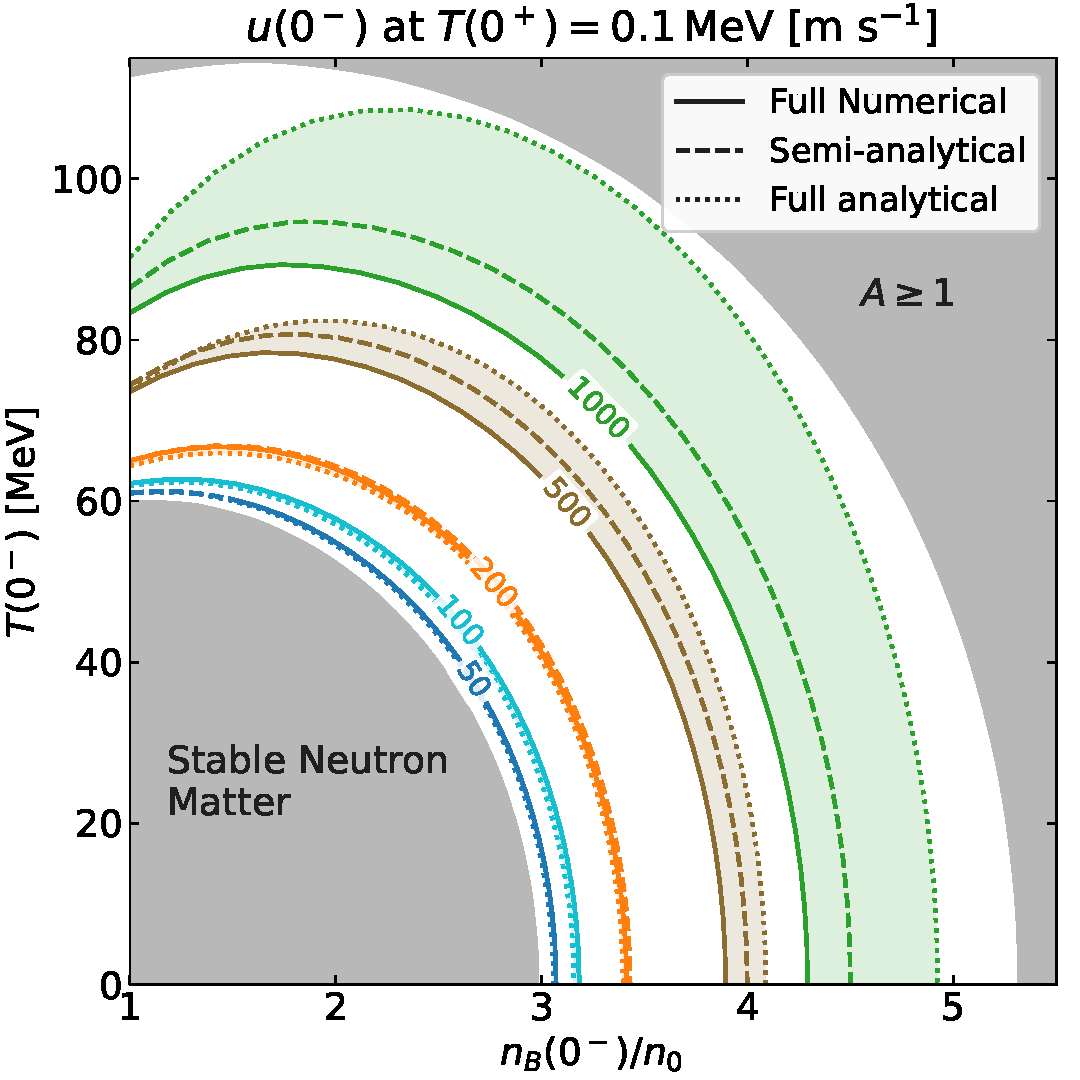
\includegraphics[width=\linewidth]{Hydrodynamical combustion/Plots/Contour-diff-meth-0.1-band.pdf}
    \caption{Comparing three methods for $T(0^+) = 0.1$ MeV. }
    \label{fig:contour-compare}
\end{figure}

\begin{figure}
    \centering
    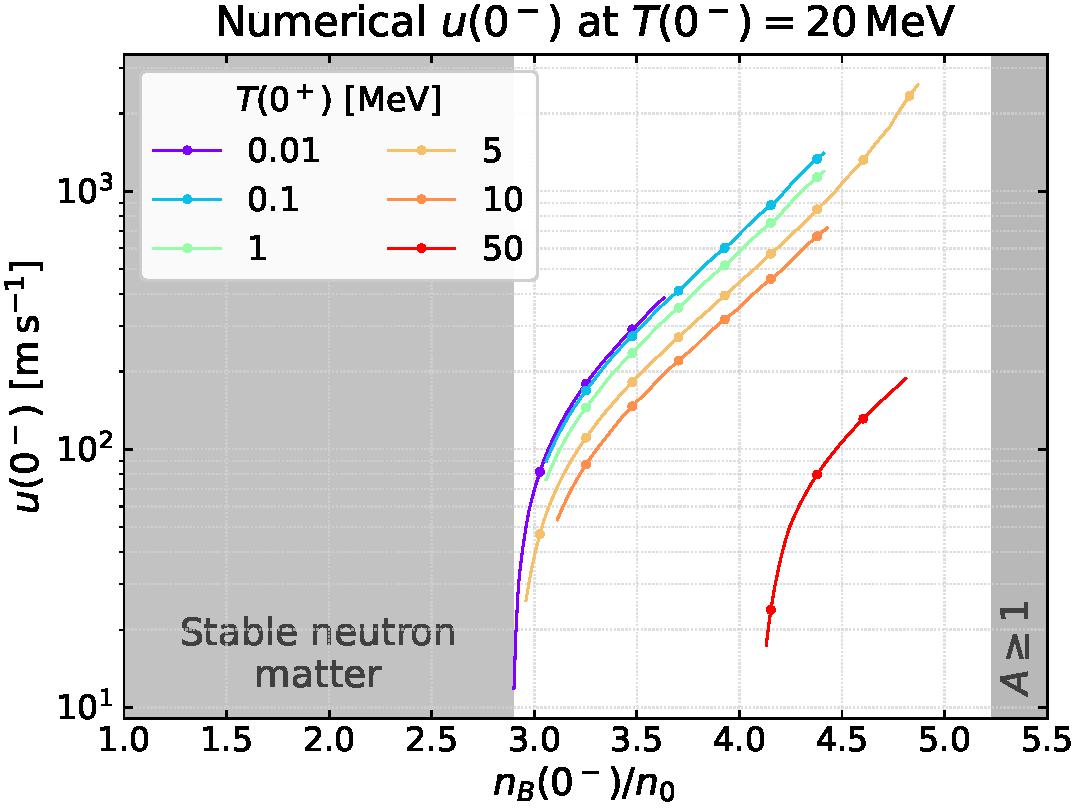
\includegraphics[width=\linewidth]{Hydrodynamical combustion/Plots/Numerical-T0plus-compare-fixT.pdf}
    \par\textbf{(a)}
    \vspace{0.5em}
    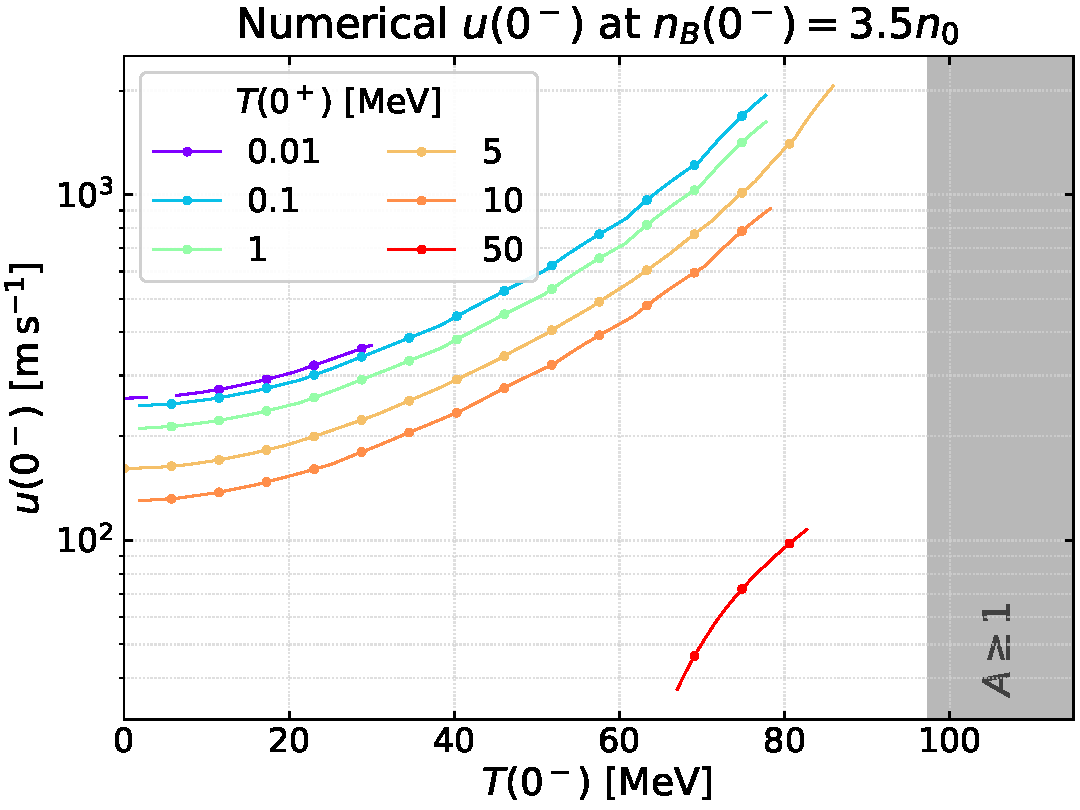
\includegraphics[width=\linewidth]{Hydrodynamical combustion/Plots/Numerical-T0plus-compare-fixnB.pdf}
    \par\textbf{(b)}
    \caption{Dependence of the numerical phase-boundary speed on the prescribed interface temperature $T(0^+)$.
    Panel (a) shows $u(0^-)$ as a function of $n_B(0^-)$ at fixed $T(0^-)=20\,\MeV$, while panel (b) shows $u(0^-)$ as a function of $T(0^-)$ at fixed $n_B(0^-)=3.5n_0$.
    The velocity axis is logarithmic, the markers denote the numerical slice samples, and the line color runs from colder (purple and blue) to hotter (red) values of $T(0^+)$.
    The gray regions are excluded in the corresponding slice by stable neutron matter or by $A_{\rm adb}\geq1$.}
    \label{fig:numerical-contour-compare}
\end{figure}

\mgacom{If we want to keep this appendix then we should flesh it out with some info about how to solve the equations, e.g. about shooting with trial values of $u(0^-)$ to find the right value.}

\JS{We solve Eq.~\eqref{eq:reduced_BVP} at fixed temperature in the isothermal case, or at fixed energy flux \eqref{eq:energy_conservation} in the adiabatic case.}
We compactify the semi-infinite quark region using
\begin{equation}
 x=-L_0\ln(1-s)\,,
 \qquad
 0\leq s\leq1-\epsilon_{\rm tail}\,,
\label{eq:compact_coordinate}
\end{equation}
where $L_0$ is fixed from the initial interface diffusion--reaction scale.
The result is checked for stability under changes of both $L_0$ and
$\epsilon_{\rm tail}\,.$  We first attempt the requested $a(0^+)$ directly;
if necessary, we continue from a smaller interface fraction and use each
converged profile as the initial guess for the next step.  States with negative
temperature, nonpositive density, a failed equation-of-state closure, or
nonphysical transport coefficients are rejected.
\JS{For the isothermal and adiabatic cases,} these profiles provide the numerical reference against which the \mga{analytic} results in Eqs.~\eqref{eq:speed_isothermal} and \eqref{eq:speed_modified}, respectively, are tested.

\section{Local thermal equilibrium}
\label{sec:thermal-equilibrium}

\LBcom{We might be able to turn this into a sentence in the main body.}However, $T(0^+)=0$ lies outside the validity of the present diffusion treatment.
As $T(0^+)\to0\,,$ the quark mean free path $\lambda^{\rm mfp}_Q$ diverges, so quark matter cannot remain in local thermal equilibrium (LTE) across a conversion layer with a finite variation scale.
Requiring the mean free path to remain shorter than the scale on which the diffusion coefficient changes,
\begin{equation}
 \lambda^{\rm mfp}_Q=3D_K
 <
 \frac{D_K}{|dD_K/dx|}\,,
\label{eq:LTE_condition}
\end{equation}
and using the constant-pressure trajectory and interface gradient gives
\begin{equation}
 5u(0^-)\Bratio a(0^+)[1-a(0^+)]
 < A_{\rm adb}^2-a^2(0^+)\,.
\label{eq:LTE_inequality}
\end{equation}
The LTE-limited composition is obtained by saturating this inequality,
\begin{equation}
 A_{\rm adb}^2-\left[a^{\rm LTE}(0^+)\right]^2
 =
 5\Bratio u(0^-)a^{\rm LTE}(0^+)
 \bigl[1-a^{\rm LTE}(0^+)\bigr]\,,
\label{eq:LTE_cutoff}
\end{equation}
with $u(0^-)$ evaluated at $a(0^+)$ from
Eq.~\eqref{eq:speed_modified}.

Finally, the full numerical solutions confirm the scale estimate: across the conversion layer, the relative variations of $n_B$ and $P$ are typically no larger than $10^{-10}$ and $10^{-12}\,,$ respectively.  
The \mga{analytic} approximation removes variation that is numerically invisible while retaining the composition and temperature profiles that set the conversion rate.



% ---- Bibliography at the very end so it covers main + SM ----
\bibliographystyle{JHEP}
\IfFileExists{reflist.bib}{\bibliography{reflist}}{\bibliography{../reflist}}

\iffalse
% =======================
%  SUPPLEMENTAL MATERIAL
% =======================
\clearpage
\onecolumngrid

\begin{center}
\textbf{\large Supplemental Material}
\end{center}
\fi


\end{document}


\JS{
\subsection{Thermal conductivity}

Currently we are setting $T(0^+) = 0$ exactly to maximize velocity. Although this can be done in the analytical or analytical approach, numerically I kept running into difficulties. I think now I have a better understanding: $T(0^+) = 0$ leads to $D_K(0^+)\to \infty$ and $D_K^{-1}(0^+) = 0$, which according to Eq.~\eqref{eq:reduced_BVP}, leads to $n_K'(0^+) = 0$. Although there's no infinities and everything seems fine, zero initial condition in derivatives is what people call non-Lipschitz initial condition. 

Why this is problematic? To break it down, this is what the numerical solver sees for $T(0^+) = 0$:
\[
\begin{aligned}
& \dfrac{dn_K}{dx}(0) \equiv \frac{n_K(\delta) - n_K(0)}{\delta} = \frac{u n_K - j_K}{D_K}(0) = 0\\
& \dfrac{d j_K}{dx}(0)\equiv \frac{j_K(\delta) - j_K(0)}{\delta} = -\Gamma_K(0)\neq 0
\end{aligned}
\]
after some rearrangements, we get
\[
n_K(\delta) = n_K(0)\,,\quad j_K(\delta) = j_K(0) - \Gamma_K\cdot \delta
\]
So $n_K(\delta) = n_K(0)$, which is sensitive to the step size $\delta$. This means the solver can return two solutions that numerically solves the equations, but they look different: their $n_K$ profile have different plateau length in the beginning. These two solutions can have $u(0^-)$ and $j_B$ differ by 20\% . 

So to resolve this, I have several plans:
\begin{itemize}
    \item cheapest: when numerically solving the set of equations, don't put in exactly zero $T(0^+)$; instead choose a sufficiently small quark matter initial temperature, say $T(0^+) = 0.01$ MeV and spend a sentence or two maybe at the $z(t)$ part explaining thermal conductivity is an interesting future research direction.
    \mgacom{Yes I prefer this approach. You need to make $T(0^+)$ small enough so that the speed no longer depends on it noticeably. Maybe that already happens for values above $0.01\,\MeV$.}
    \item minimal thermal conductivity, where we don't add another full ODE to solve, but just model the thermal conductivity ODE, and just integrate it across $x=0$ to place a lower bound on $T(0^+)$
    \item full thermal conductivity modeling. To do this we need to replace the current energy conservation equation $d(h\gamma u)/dx = 0$ by a second order ODE similar to what we have for $n_K$ right now:
\[
\frac{d}{dx}\Big(h\gamma u - \kappa_{\rm th}\frac{dT}{dx}\Big) = -Q_\nu
\]


\hide{
\section{Heat Transport}
\label{sec:heat_transport}
\LBcom{This entire appendix needs clarification.}

The nonadvective thermal current $q_{\rm th}^\mu$, the term that describes heat flowing relative to the fluid, satisfies $U_\mu q_{\rm th}^\mu=0$ and is purely spatial in that frame~\cite{Eckart:1940te,Harutyunyan:2023nvt}.
\LBcom{isn't $q$ only spatial in the rest frame of the fluid?}
\JScom{In Eckart's heat law, Eq.~\eqref{eq:eckart_heat_flux}, $(g^{\mu\nu}-U^\mu U^\nu)\nabla_\nu T=(g^\mu_{\;\nu}-U^\mu U_\nu)\nabla^\nu T$.
The operator $g^\mu_{\;\nu}-U^\mu U_\nu$ projects the temperature gradient into the local rest space orthogonal to $U^\mu$.
The acceleration term is also orthogonal to $U^\mu$, since $U_\mu\nabla_\alpha U^\mu=\tfrac12\nabla_\alpha(U_\mu U^\mu)=0$.
Thus $q^\mu_{\rm th}$ is purely spatial in the baryon fluid rest frame, not generally in the phase boundary rest frame.}


For stationary profiles in which the heat current adjusts much faster than the conditions experienced by the fluid change \LBcom{What conditions?}, we use the first-order Eckart heat law~\cite{Eckart:1940te,Lopez-Monsalvo:2010oeo,Lander:2018cvq},
\begin{equation}
\begin{aligned}
q_{\rm th}^{\mu}=\kappa_{\rm th}\bigl[&
(g^{\mu\nu}-U^\mu U^\nu)\nabla_\nu T\\
&-T U^\alpha\nabla_\alpha U^\mu\bigr]\ ,
\end{aligned}
\label{eq:eckart_heat_flux}
\end{equation}
where $\kappa_{\rm th}\geq0$ is the thermal conductivity.
The first term is the temperature gradient projected into the local fluid rest space; the second is the relativistic acceleration correction.

We impose steady planar flow in flat spacetime, so all fields depend only on $x$.
With $U^\mu=(\gamma,u,0,0)$, orthogonality gives $q_{\rm th}^0=u q_{\rm th}^x/\gamma$, and Eq.~\eqref{eq:eckart_heat_flux} gives
\begin{equation}
q_{\rm th}^x=-\kappa_{\rm th}\left[(1+u^2)\frac{dT}{dx}
+T u\frac{du}{dx}\right]\ .
\label{eq:eckart_heat_flux_steady}
\end{equation}
Baryon conservation gives $du/dx=-(u/n_B)\,dn_B/dx$, so the acceleration term is of order $u^2$ and is negligible because $u$ and $n_B$ are nearly constant on either side of the boundary.
Keeping the transport terms to leading order in $u\sim3\times10^{-7}$ ($u^2\sim10^{-13}$), while retaining the relativistic form of the ideal-fluid fluxes, is consistent with the adiabatic numerical check of relative $n_B$ and $P$ variations below $10^{-10}$ and $10^{-12}$, respectively (Appendix~\ref{sec:thermal-equilibrium}).
This gives Fourier's law,
\begin{equation}
    q_{\rm th}^x\simeq-\kappa_{\rm th}\frac{dT}{dx}\ ,
    \label{eq:fourier_heat_flux}
\end{equation}
The minus sign directs heat toward lower temperature.
In quark matter, $\kappa_{\rm th}$ is determined by quark scattering~\cite{Heiselberg:1993cr}.%; it is a separate transport coefficient from the K diffusion coefficient $D_K$.

\JS{We use independent density-gradient Fick and temperature-gradient Fourier laws, neglecting thermodiffusion (the Soret effect) and composition-driven heat flow (the Dufour effect).
The Fick law uses a gradient of $n_K$ rather than of $\mu_K/T$.
We also neglect energy carried by K interdiffusion, so the nonadvective energy current in Eq.~\eqref{eq:stress_tensor} is approximated by conduction alone.
These are additional transport assumptions, not consequences of slow flow, and they are retained in both thermal limits.
The thermal limits below are taken after this slow-flow reduction; exactly constant $T$ does not by itself remove the acceleration term in Eq.~\eqref{eq:eckart_heat_flux_steady}.}
}


where Eq. (62) in \cite{Heiselberg:1993cr} gives a very similar expression for $\kappa_{\rm th}$ compared with $D_K$, and $Q_\nu$ is the energy taken away by neutrinos per unit time. So judging by the similarity, I assume every method: analytical, numerical, whatever we have developed for solving the $n_K$ ODE would also apply here. But the draw back of the full thermal conductivity modeling is that we are not including Urca, so this $Q_\nu$ is essentially zero in our model. We need to explain that away. 
\end{itemize}

}

